\chapter{Results}
\label{chap:results}

All experiments conducted are about assembling target polyominoes with the use of our global planner (\autoref{chap:global}).
In \autoref{sec:AFN} we analyze the effect of increasing polyomino size on planning time, rotational cost and other global planner characteristics mentioned in \autoref{sec:global_complex}.
The polyominoes used for this experiment are randomly generated, but we also evaluate the construction of manually designed polyominoes in \autoref{sec:AFTS}.
With these polyominoes, we can specifically test the assembly of targets with caves or holes, varying widths and heights, or different patterns of red and blue cubes. 
Furthermore, we experiment with different workspace sizes and aspect ratios in \autoref{sec:AFBS} and how the ratio of red and blue cubes affect the assembly of straight line polyominoes in \autoref{sec:AFNR}.

\paragraph{Option Sorting Strategies}
We run all experiments with the three option sorting strategies from \autoref{sec:connect_options},
\begin{enumerate}
	\item Minimal Distance (MIN DIST)
	\item Grow Largest Component (GROW LARGEST)
	\item Grow Smallest Component (GROW SMALLEST)
\end{enumerate}

\paragraph{Instance Generation}
For the generation of random polyominoes and initial configurations we use a seed-based pseudorandom number generator to make experiments reproducible.
That way the option sorting strategies are applied to the same set of seeds to make the results comparable.
When an initial configuration is randomly generated the number of red and blue cubes matches with the target polyomino.
Sub-assemblies in the initial configuration can occur, since the global planner is able to handle this.

\paragraph{Timeout Failure}
The global planner states a timeout failure after a planning time of $600$ seconds.
We do not time out during the simulation of local plans, so instances can exceed $600$ seconds and still be successful if the last local plan assembles the target polyomino.

\paragraph{Hardware Setup}
The experiments were done on multiple computers with the same hardware specification (\textbf{AMD Ryzen 7 5800X @ 8x3.8GHz (-4.7 GHz), 128GB RAM}) running Ubuntu 22.04.2 LTS.

%TODO key legende fuer box-whisker plots




\section{Assembly for Polyomino Size}
\label{sec:AFN}

This experiment was conducted with randomly generated initial configuration and randomly generated polyominoes of specific sizes $n$.
To maximize the variety of possible polyomino-shapes the number of red cubes is set to $n_\textit{red} = \lfloor \frac{n}{2} \rfloor$ \cite{Lu2021}.
Because of the variety, this experiment is well-suited for not only analyzing planning time and rotational-cost, but also examine $\#\textit{local}$, $\#\textit{config}$ and $|P|$.
We worked in a quadratic workspace of size $50 r_C \times 50 r_C$ and for each target size $150$ samples were taken.

\subsection{Planning Time}

\begin{figure}
	\centering
	\begin{subfigure}[b]{\textwidth}
		\centering
		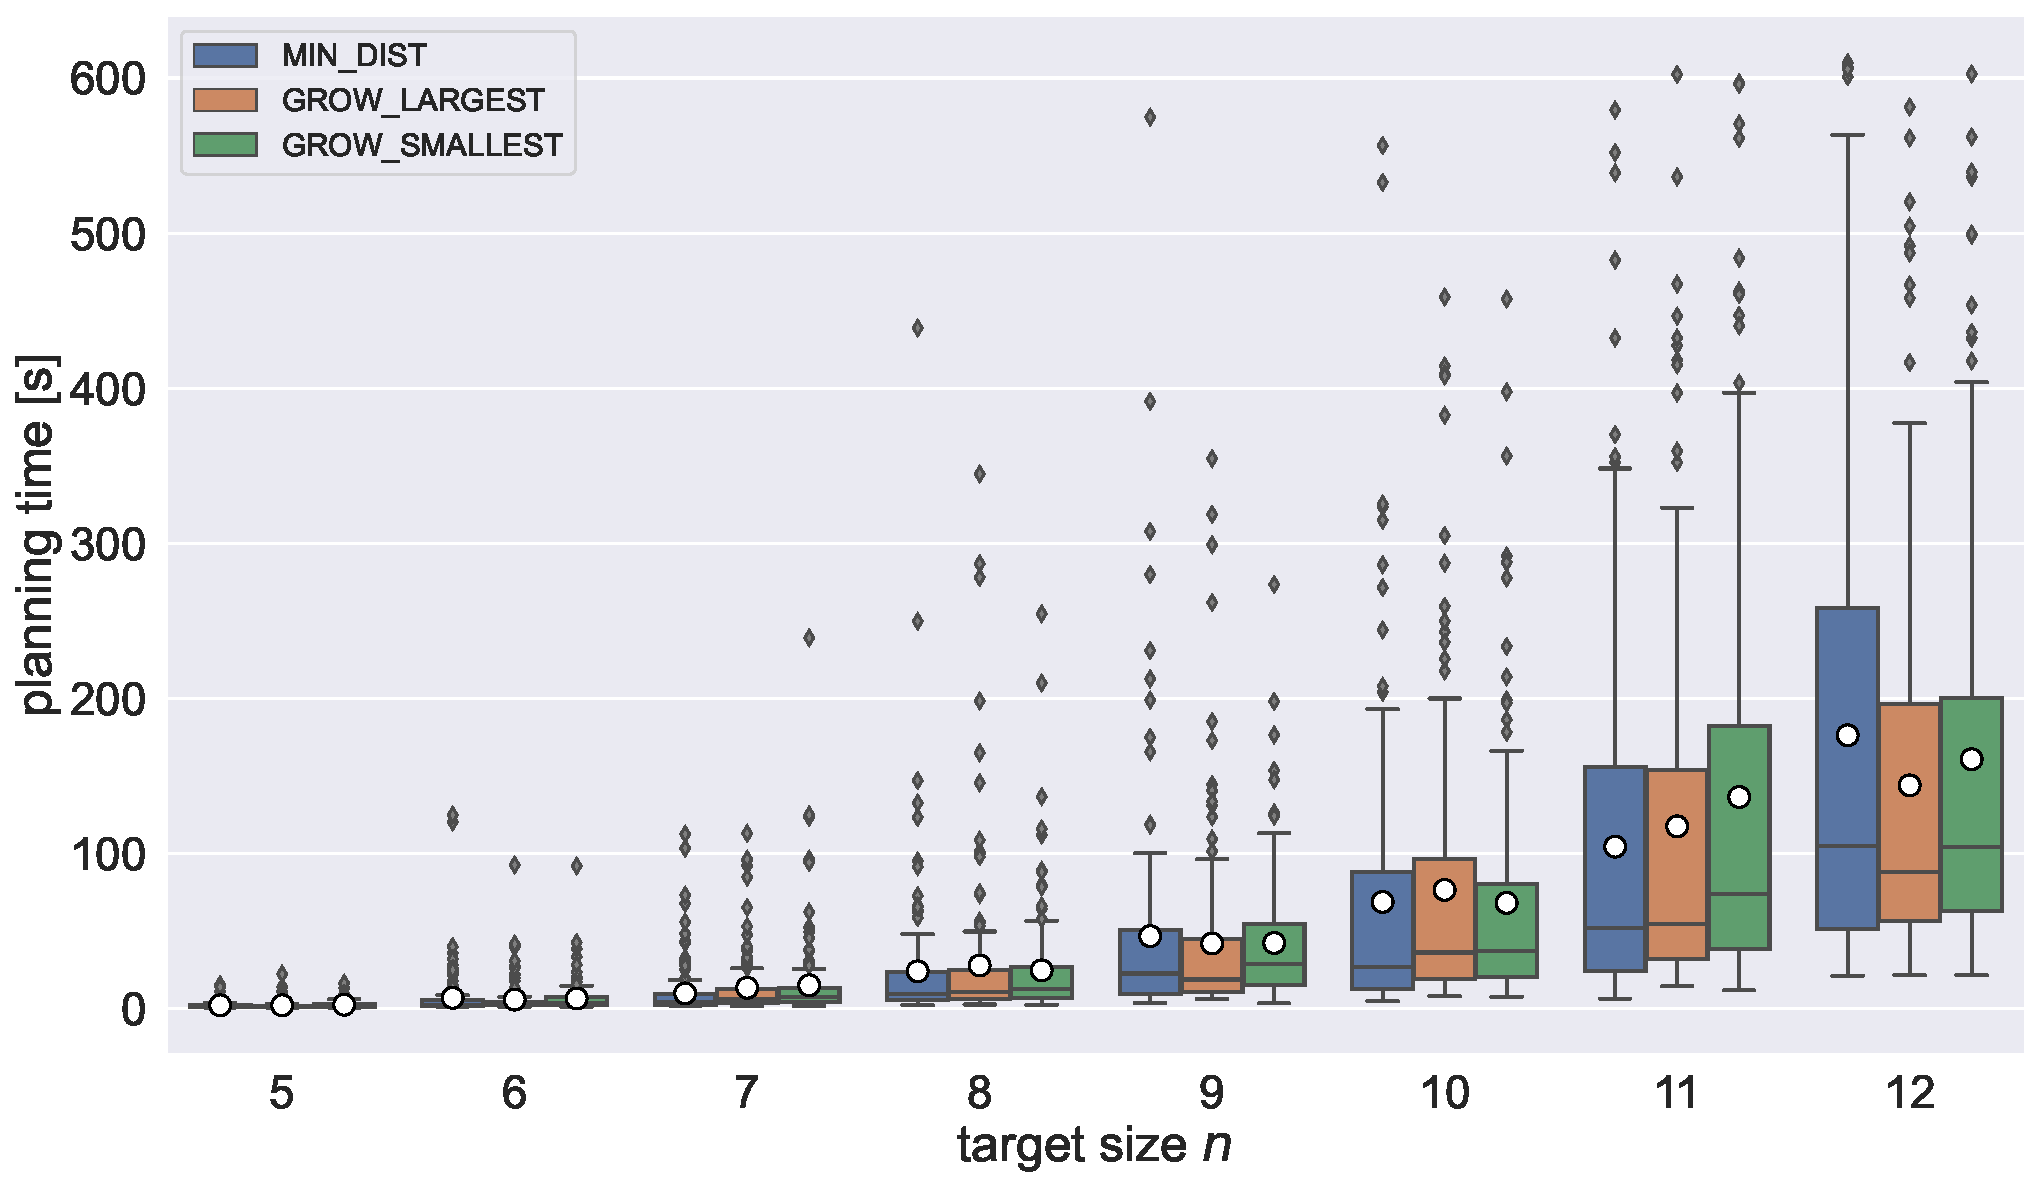
\includegraphics[width=0.9\textwidth]{figures/plots/AFN_time.pdf}
		\caption{Planning time in seconds. Only plans that did not time out are shown.}
		\label{fig:AFN_time}
	\end{subfigure}

	\begin{subfigure}[b]{\textwidth}
		\centering
		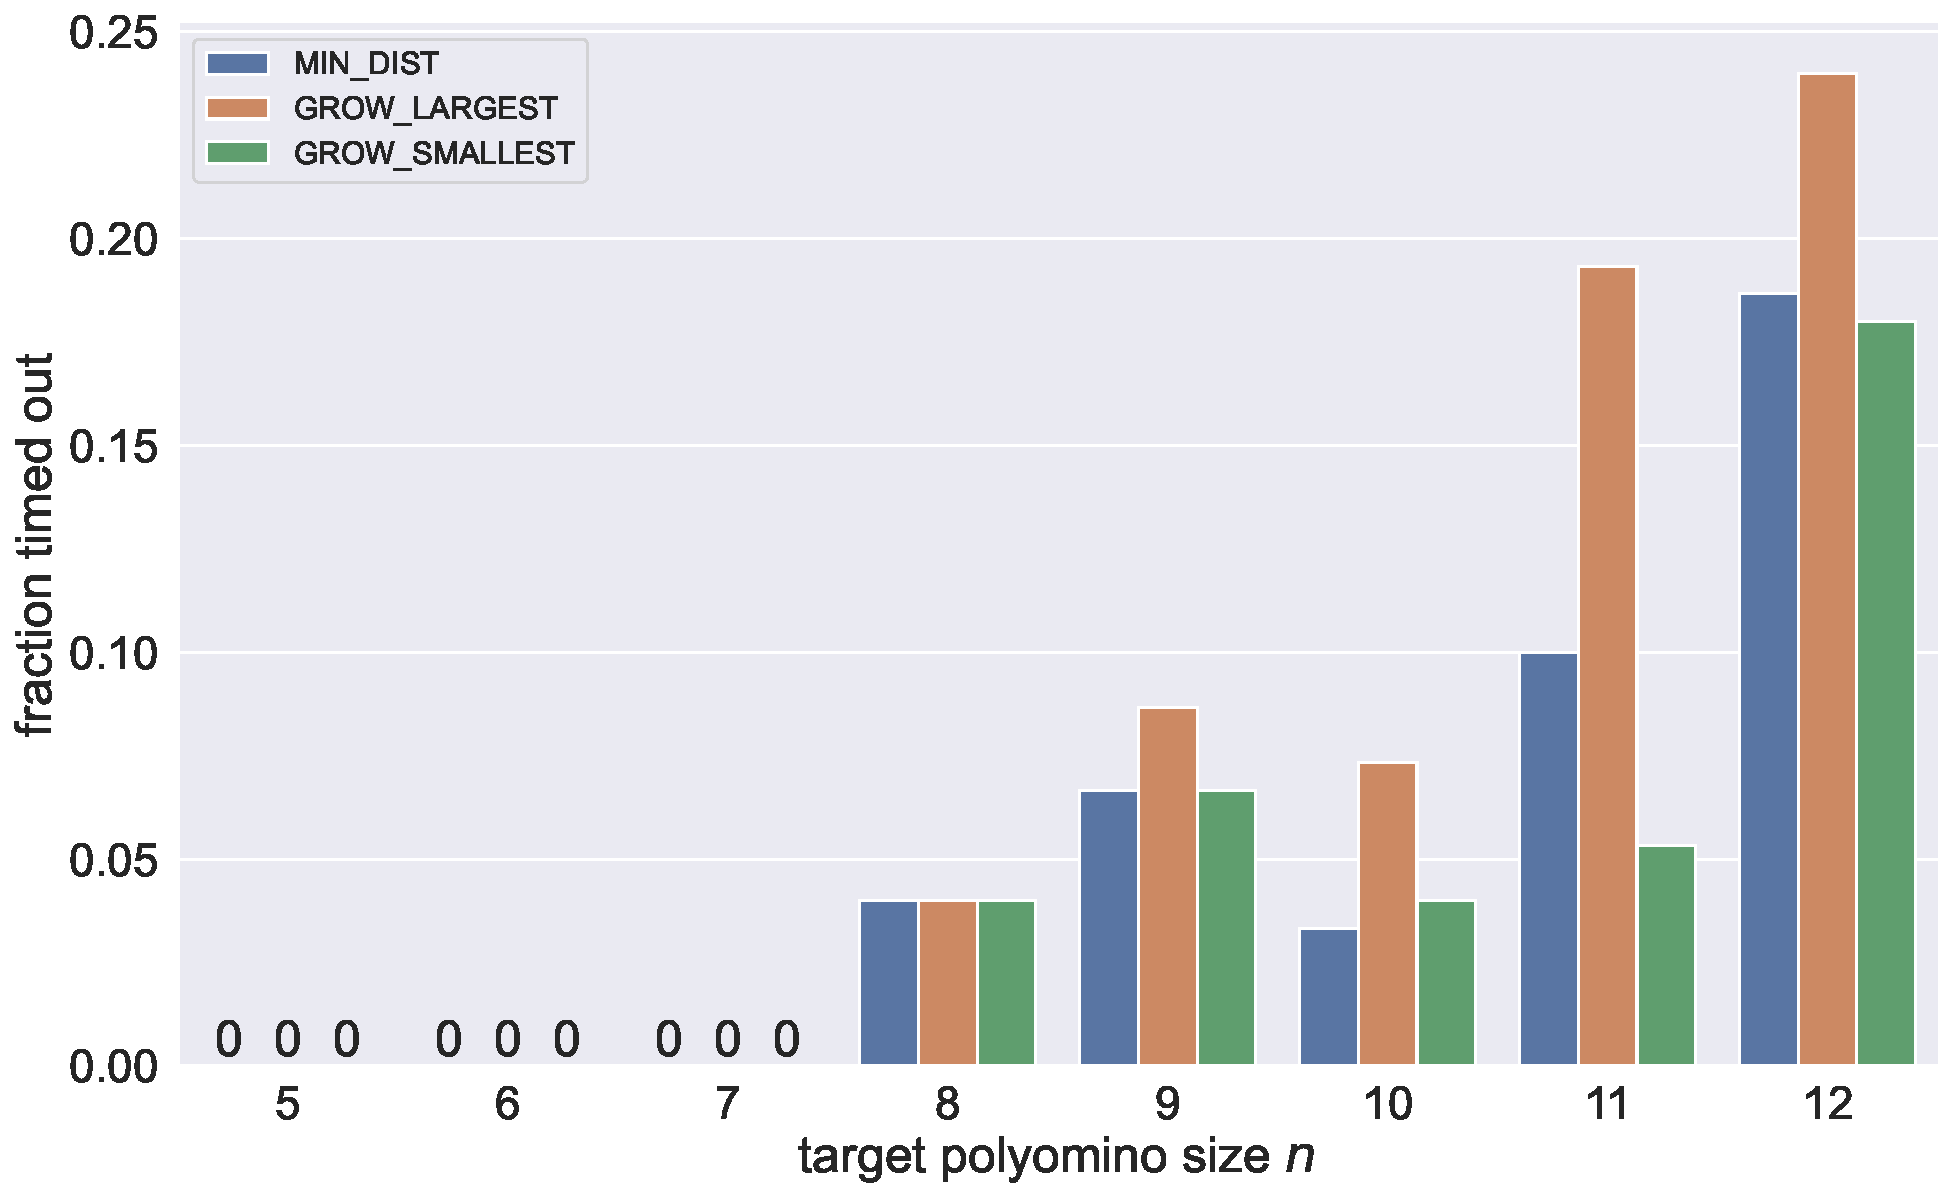
\includegraphics[width=0.9\textwidth]{figures/plots/AFN_timeout.pdf}
		\caption{Fraction of plans that timed out}
		\label{fig:AFN_timeout}
	\end{subfigure}
	\caption[Planning time and fraction timed out for different target sizes]{Planning time and fraction timed out for different target sizes $n$. All option sorting strategies are compared.}
	\label{fig:AFN_timestats}
\end{figure}

\autoref{fig:AFN_time} shows distribution of planning time and \autoref{fig:AFN_timeout} plots the fraction of timeouts during this experiment.
The construction of target polyominoes with sizes $5$ to $7$ can be planned in under $30$ seconds with just a few outliers exceeding this time.
Note the non of the instances timed out.

For target sizes above $7$ timeout failures first appear with roughly $5\%$ for $n = 8$.
The fraction of timeouts increases to $20\%$ for $n=12$.
The planning time for $n = 12$ increases to $150$ seconds on average with a median of $100$ seconds.
With increasing $n$, a wider spread of planning time can be observed.
Outliers can reach planning times close to the timeout of $600$ seconds.´

In terms of planning time the option sorting strategies make no noticeable difference.
For the fraction of timeouts, growing the largest component often exceeds the other two strategies clearly visible for $n=11$, where grow largest is at $20\%$ and the others under $10\%$ of plans timed out.


\subsection{Plan Cost}

\begin{figure}
	\centering
	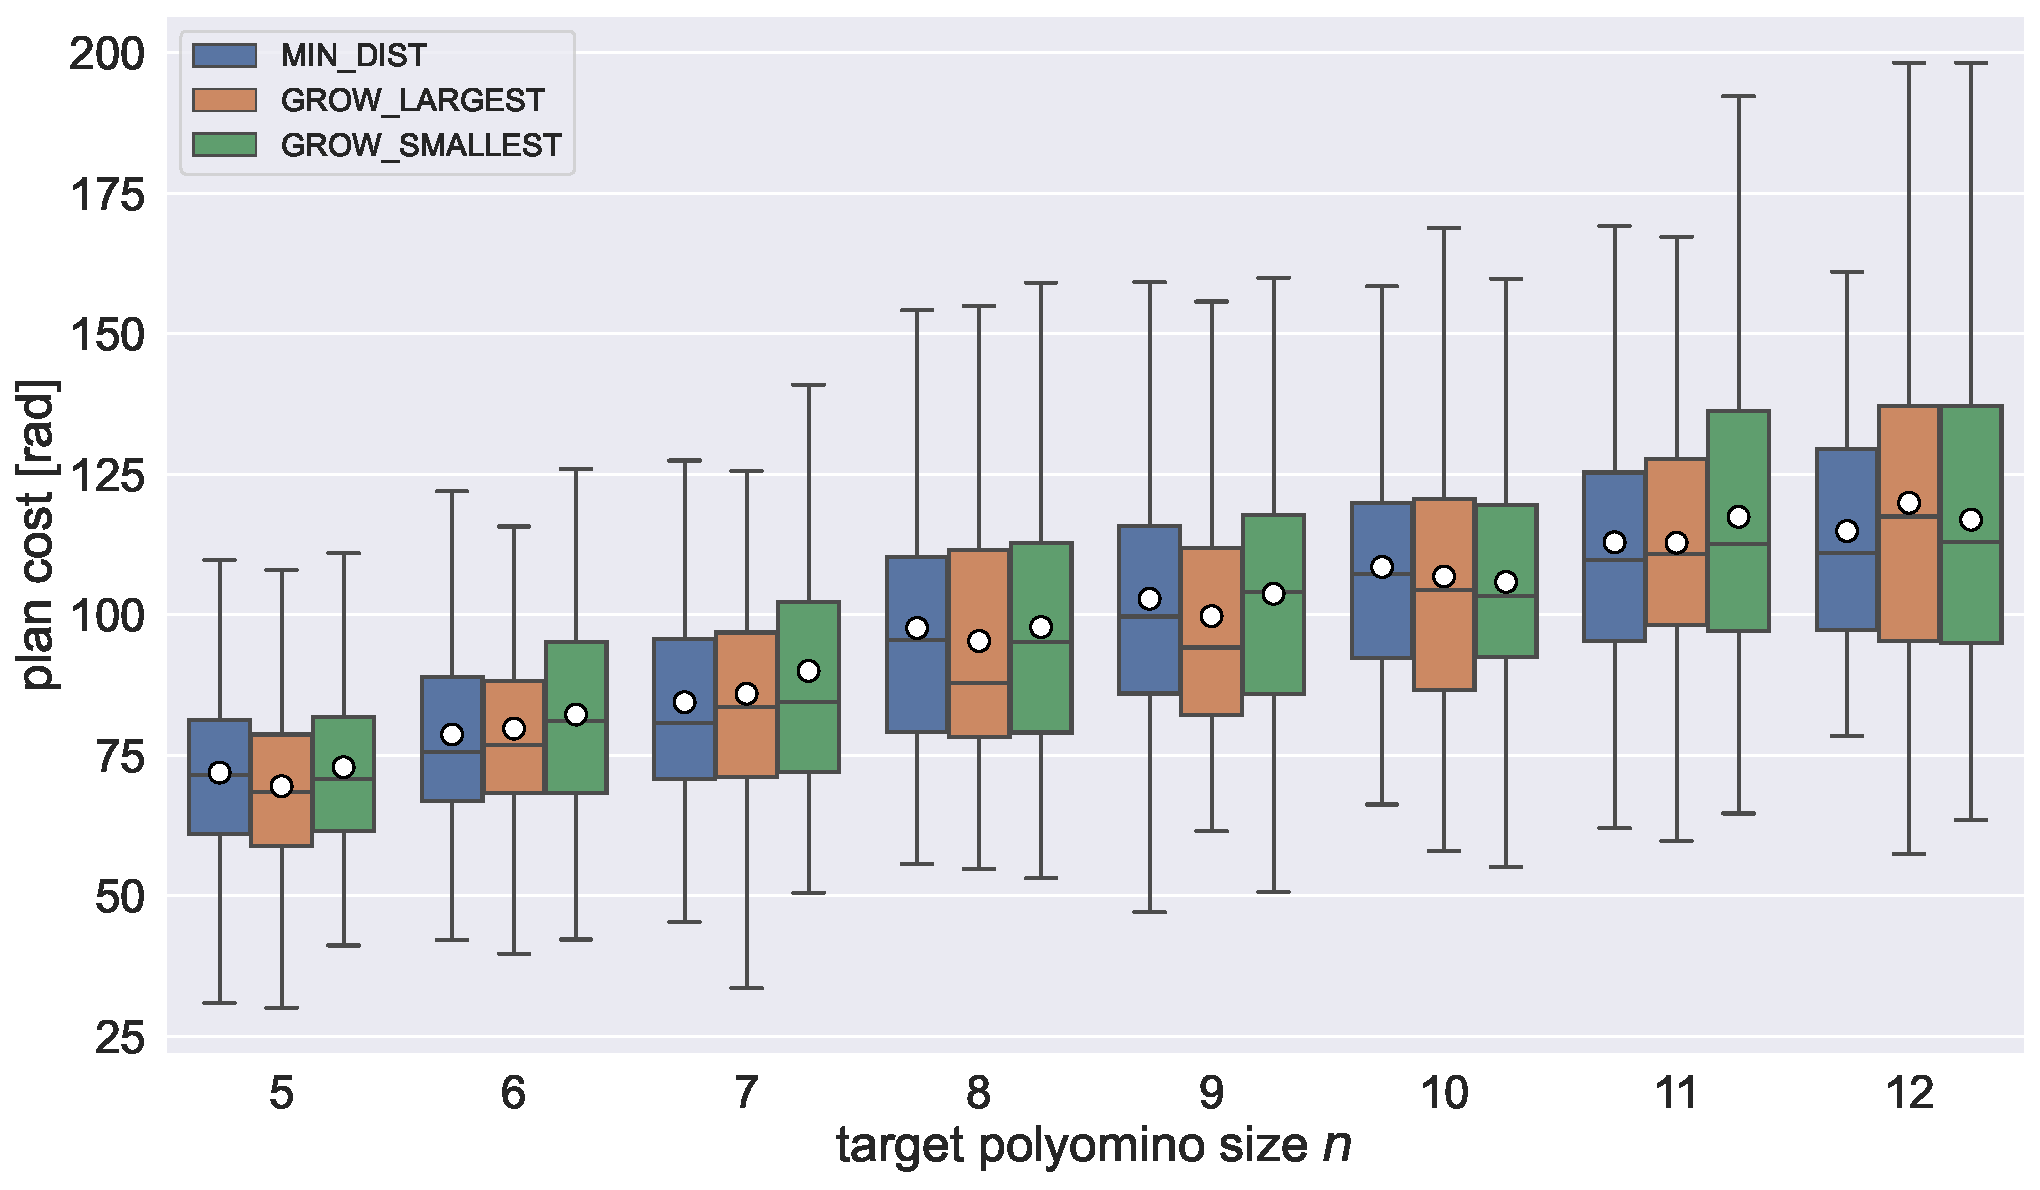
\includegraphics[width=0.9\textwidth]{figures/plots/AFN_cost.pdf}
	\caption[Plan cost for different target sizes]{Plan cost in radians of successful plans for different target sizes $n$. All option sorting strategies are compared.}
	\label{fig:AFN_cost}
\end{figure}

\autoref{fig:AFN_cost} shows the rotational cost of the resulting plans that successfully assembled the target.
The cost increase slightly for bigger polyominoes, but the gradient increases gently and seems to be flatting out for sizes $11$ and $12$.
Plan cost is generally in a range of $50$ to $150$ radians, which is the equivalent of $8$ to $24$ full longitude rotations of the magnetic field.
The different option sorting strategies do not impact the cost of a plan.

\subsection{Planning Attributes}

\begin{figure}
	\centering
	\begin{subfigure}[b]{\textwidth}
		\centering
		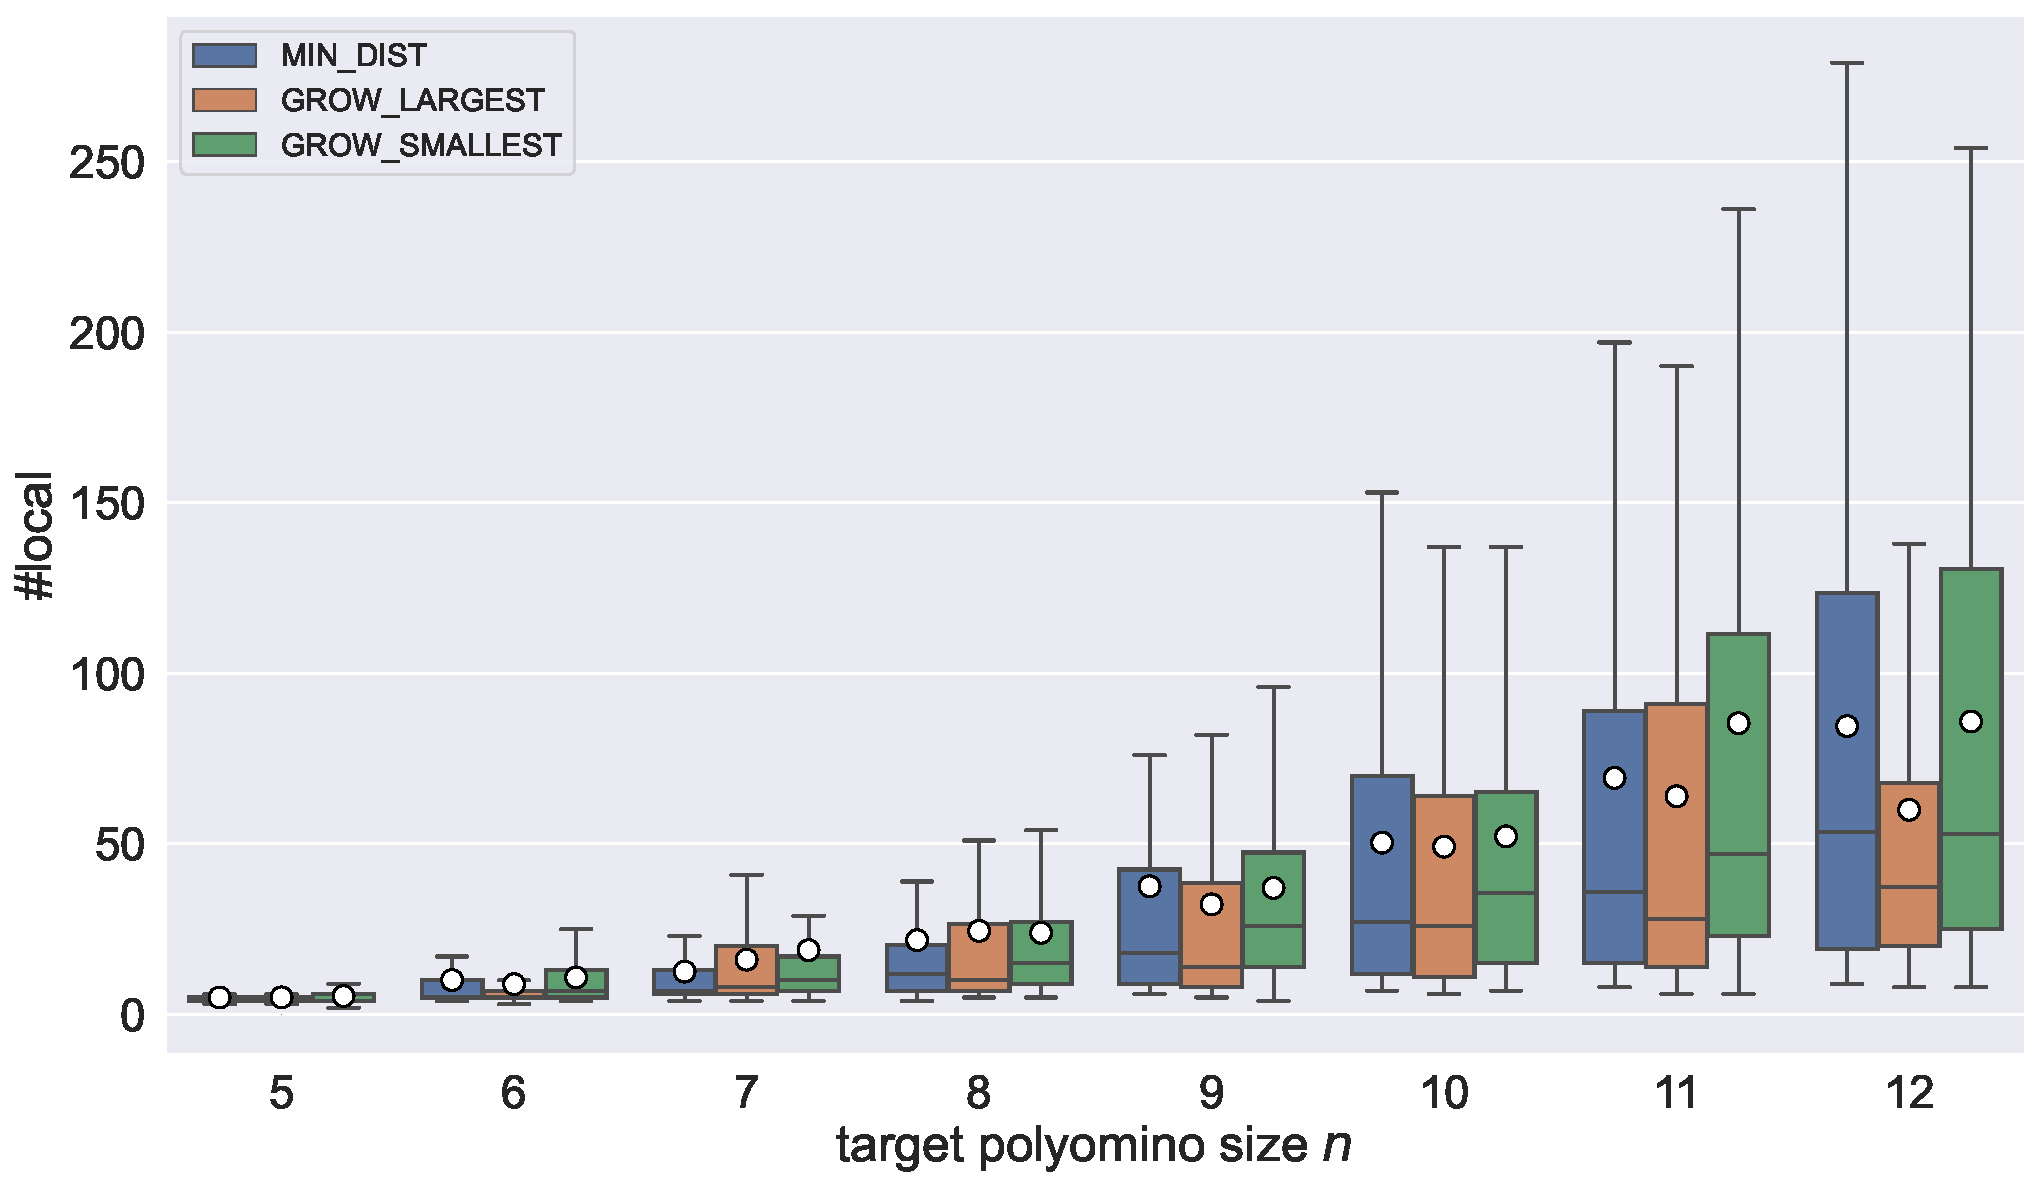
\includegraphics[width=0.9\textwidth]{figures/plots/AFN_nlocal.pdf}
		\caption{Number of simulated local plans.}
		\label{fig:AFN_nlocal}
	\end{subfigure}
	
	\begin{subfigure}[b]{\textwidth}
		\centering
		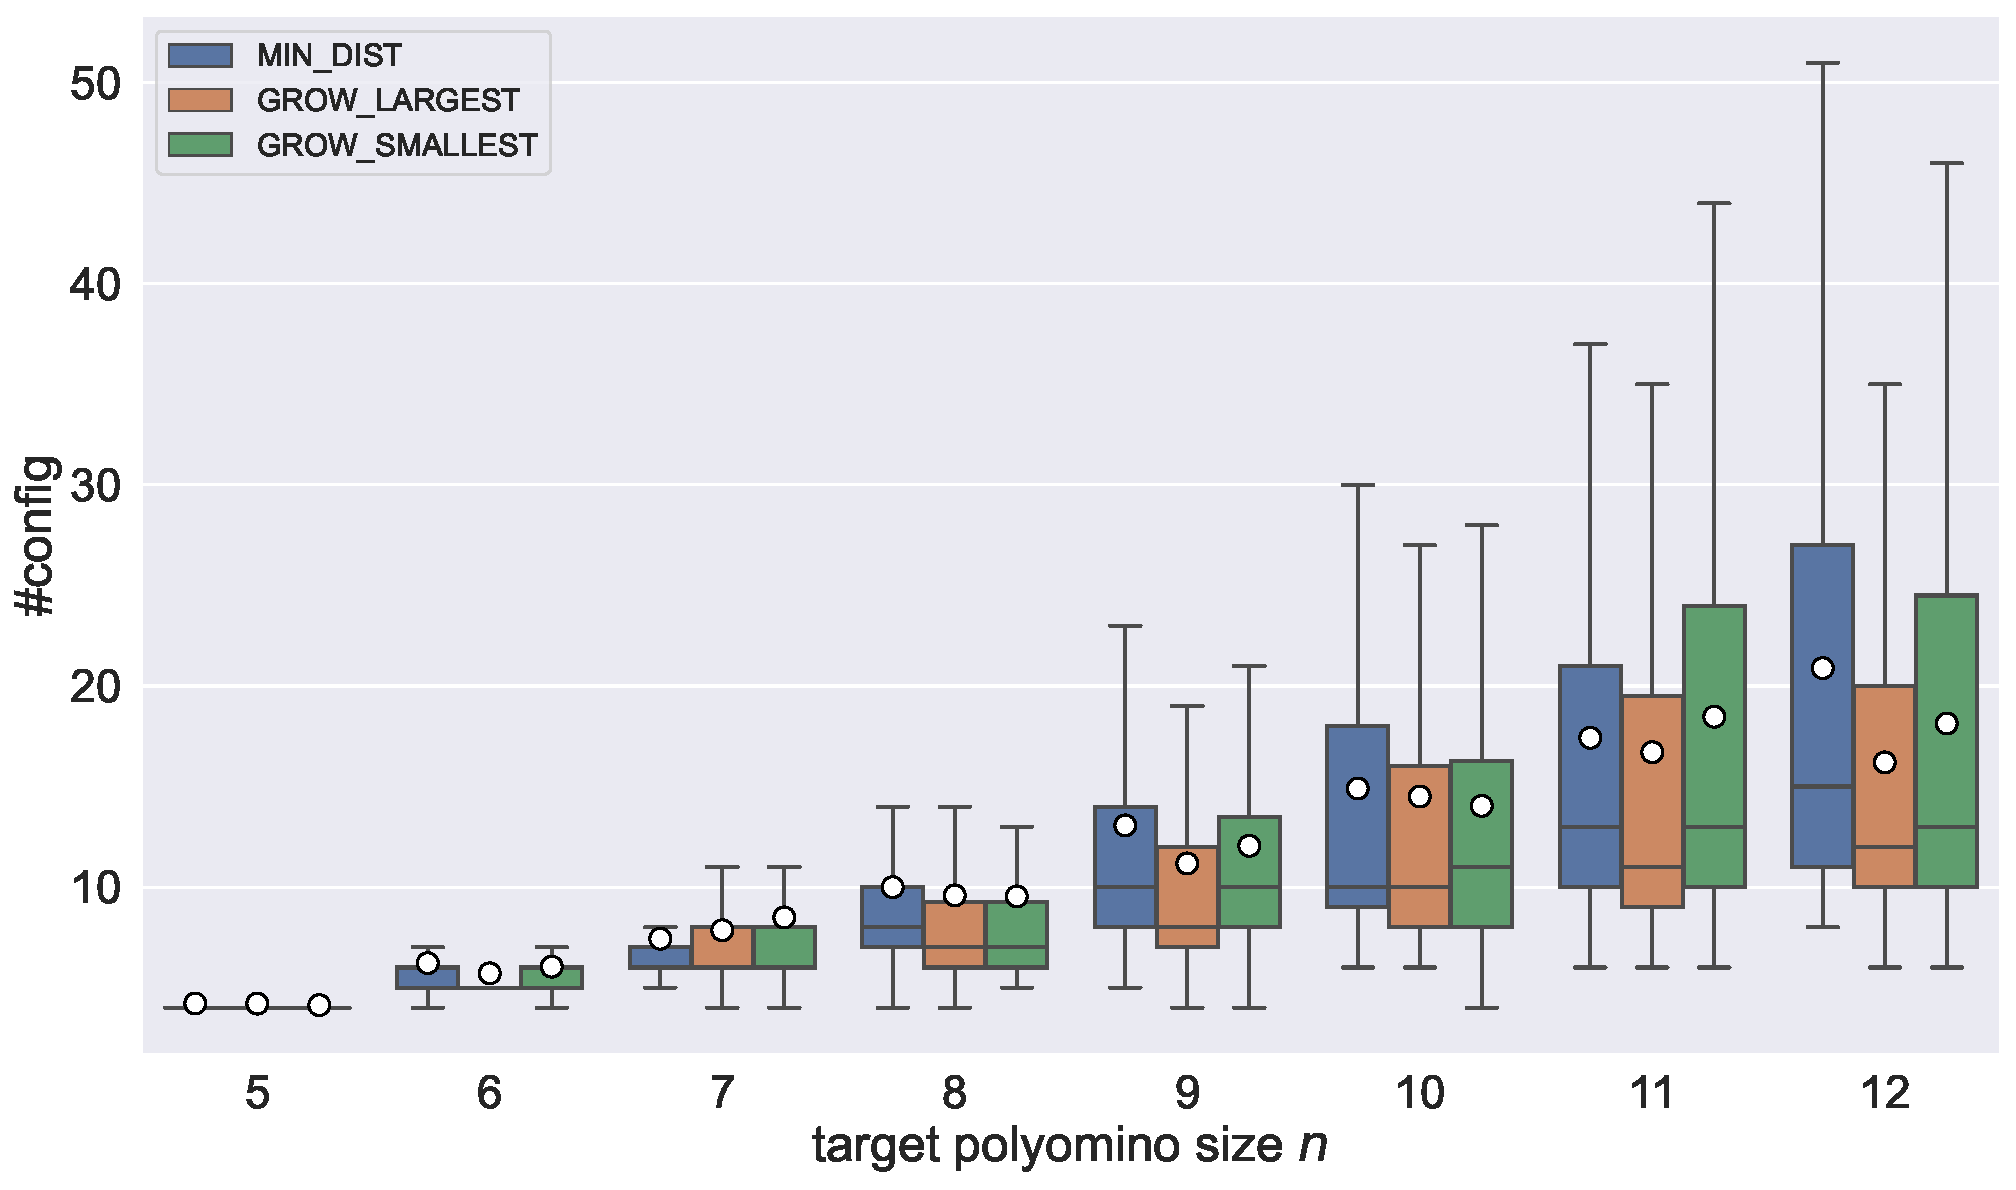
\includegraphics[width=0.9\textwidth]{figures/plots/AFN_nconfig.pdf}
		\caption{Number of explored configurations}
		\label{fig:AFN_nconfig}
	\end{subfigure}
	\caption[$\#\textit{local}$ and $\#\textit{config}$ for different target sizes]{Number of simulated local plans $\#\textit{local}$ and number of explored configurations $\#\textit{config}$ for different target sizes $n$. Only plans that did not time out are shown and outliers are omitted for better readability. All option sorting strategies are compared.}
	\label{fig:AFN_planstats}
\end{figure}

\begin{figure}
	\centering
	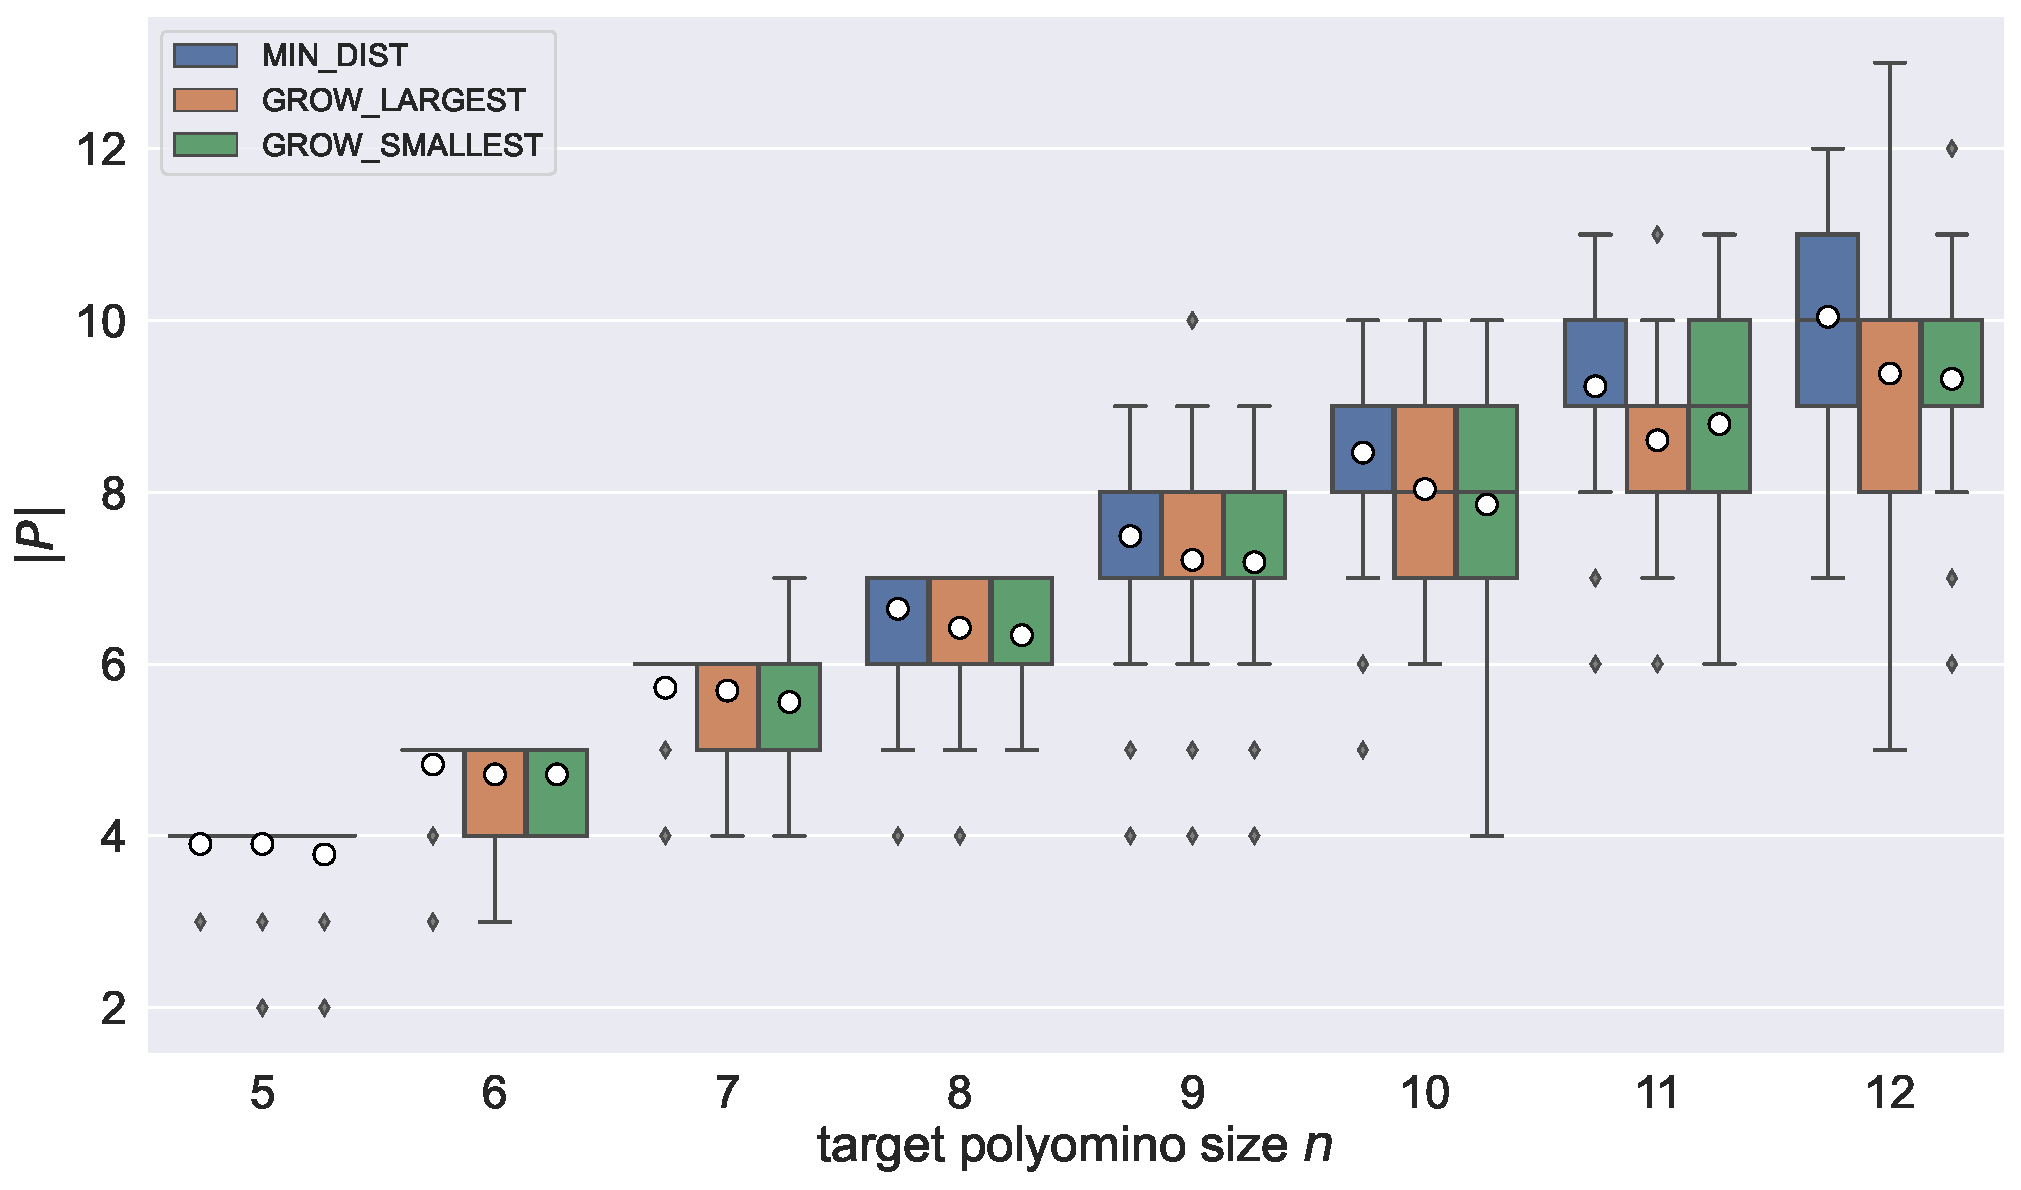
\includegraphics[width=0.9\textwidth]{figures/plots/AFN_ltg.pdf}
	\caption[Local plans in plan stack for different target sizes]{Local plans in plan stack $|P|$ for different target sizes $n$. Only successful plans are shown and all option sorting strategies are compared.}
	\label{fig:AFN_ltg}
\end{figure}


We analyze the number of simulated local plan $\#\textit{local}$ and the number of explored configuration $\#\textit{config}$ in \autoref{fig:AFN_planstats}.
The number of local plans contained in the plan stack of the resulting global plan $|P|$ is evaluated in \autoref{fig:AFN_ltg}.
When a plan times out it is not possible to predict how many more local plan or configurations would have to be explored to assemble the target.
In that case $\#\textit{local}$ and $\#\textit{config}$ just show how many local plan and configurations can be explored within the timeout.
Numbers can reach values up to $\#\textit{local} = 1200$ and $\#\textit{config} = 300$, but all plans that timed out are omitted in the plots of \autoref{fig:AFN_planstats}.

$\#\textit{local}$ increases for bigger target polyominoes.
On average the realistic best case of $n-1$ local plans (\autoref{sec:global_complex}) is exceeded.
For $n=8$ there were $25$, for $n=10$ about $50$ and for $n=12$ roughly $75$ local plans simulated on average.
For all target polyomino sizes the majority of instances is below the average, although some instances can reach up to $250$ local plans.

The same goes for $\#\textit{config}$.
The averages exceeds the realistic best case of $n$, for example $16$ with $n=12$.
In this example the global planner encountered at least $4$ dead ends during planning.
The small numbers of $\#\textit{config}$ show that the depth first search approach is able to assemble polyominoes by only exploring a small portion of the whole configuration space.

For the majority of instances $|P| = n-1$, but layer skipping can be observed whenever $|P| < n-1$.
Surprisingly we observe instances with $|P| > n-1$.
This should not be possible when assembling with a TCSA graph.
The only explanation for this is that polyominoes break during simulation and create polyomino sets, which are at the same or a lower depth then the initial set.
This effect becomes more frequent for $n \geq 9$.

In terms of the option sorting strategies the only noticeable difference is that growing the largest component tends to have slightly lower value of $\#\textit{config}$.



\section{Assembly for Custom Polyominoes}
\label{sec:AFTS}

\begin{figure}
	\centering
	\begin{subfigure}[b]{\textwidth}
		\centering
		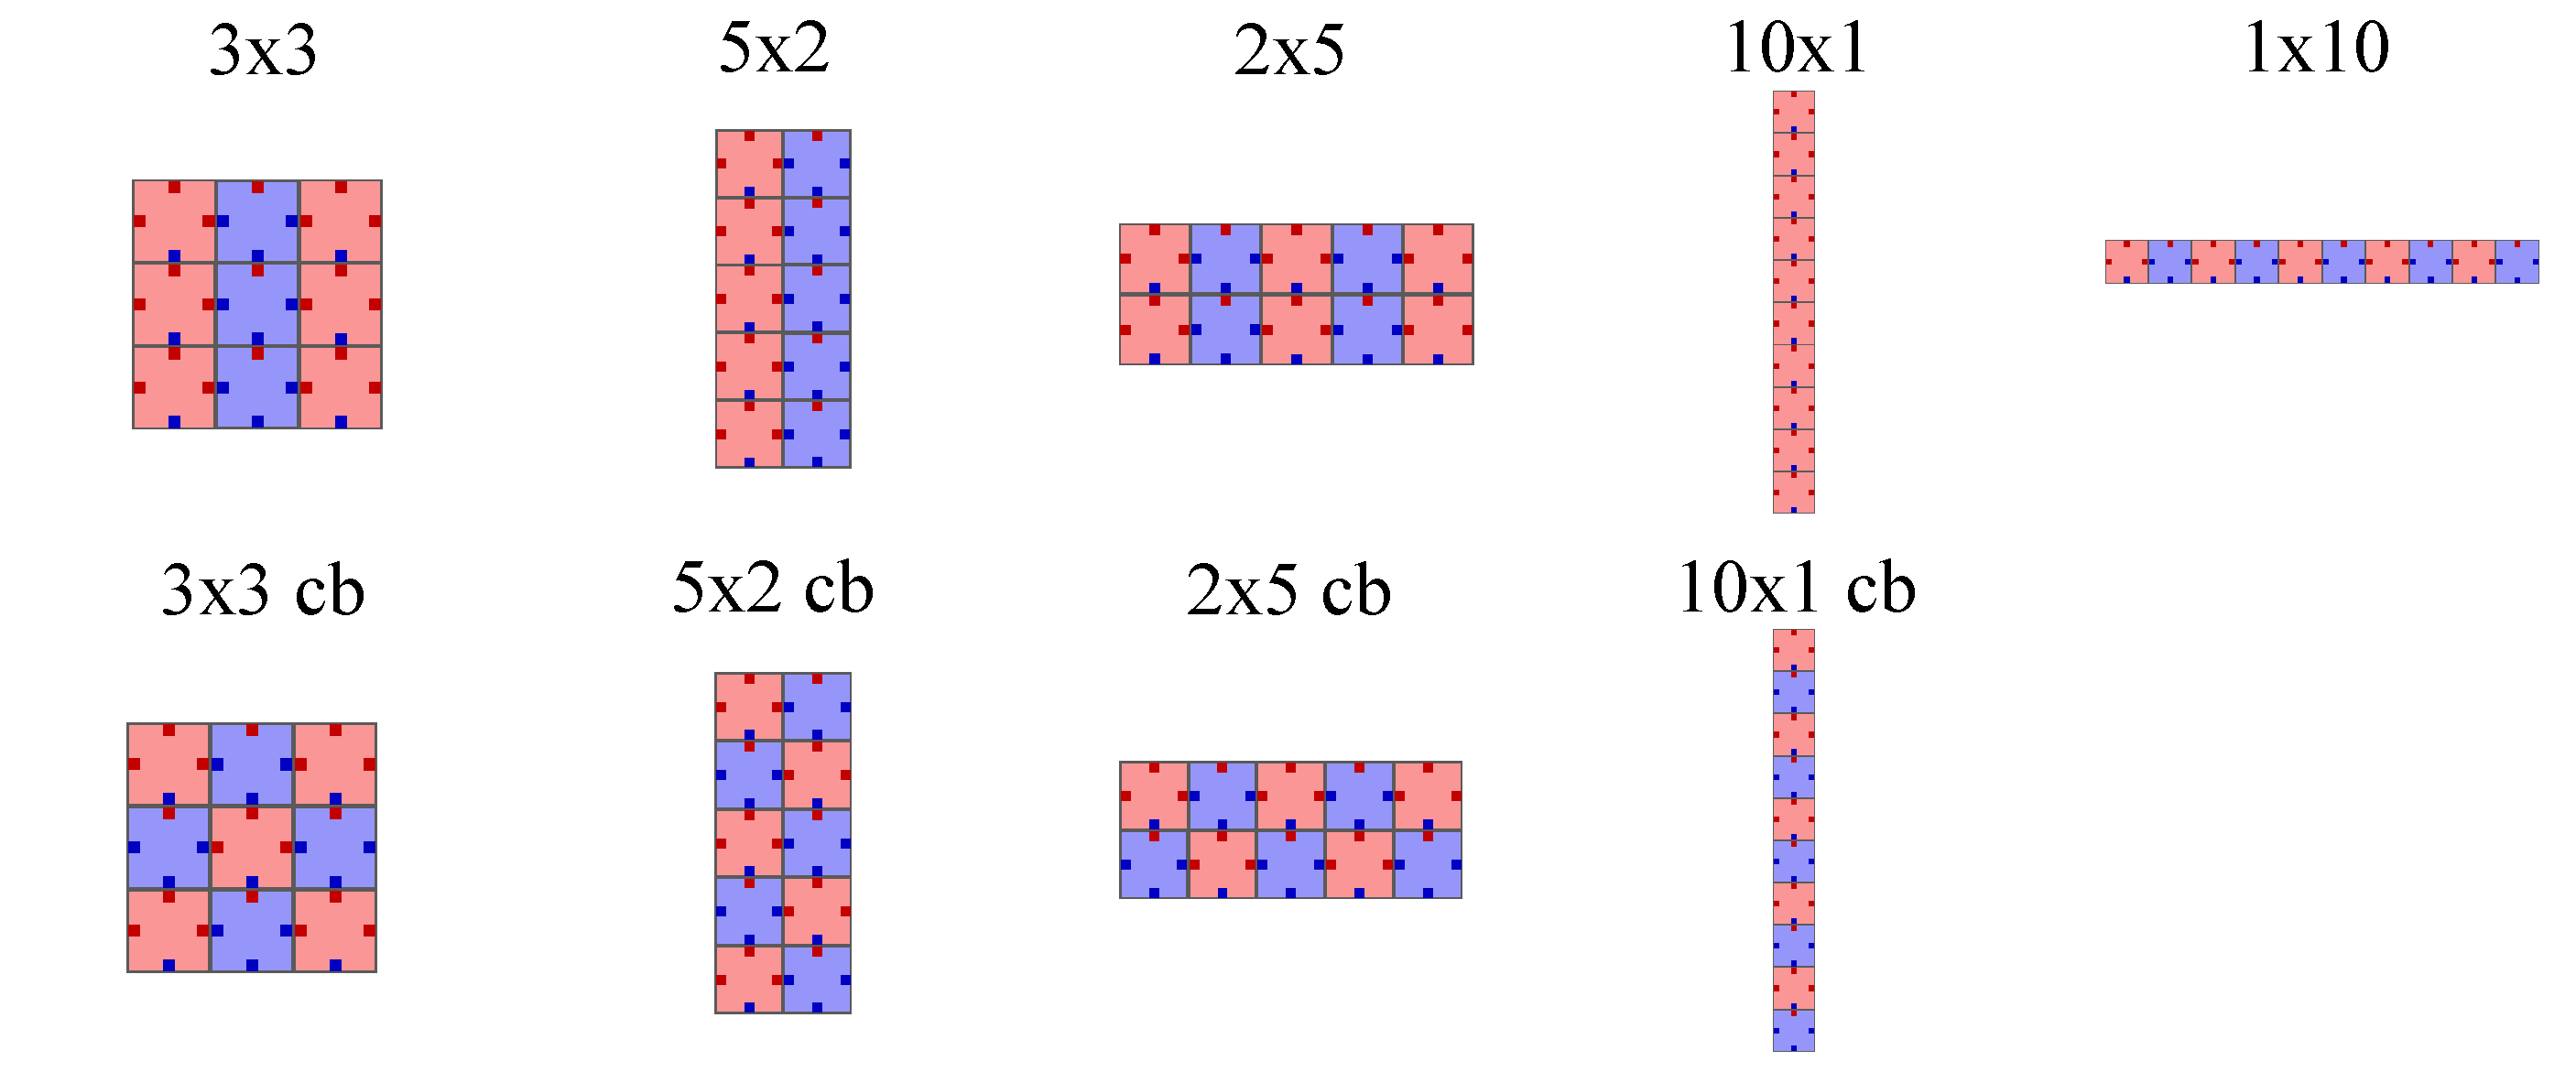
\includegraphics[width=0.8\textwidth]{figures/AFTS_cb_shapes.pdf}
		\caption{Rectangular polyominoes evaluated in \ref{sec:w/h_pattern}. The checkerboard pattern is labeled with ``cb''. \hfill}
		\label{fig:AFTS_cb_shapes}
	\end{subfigure}
	\begin{subfigure}[b]{\textwidth}
		\centering
		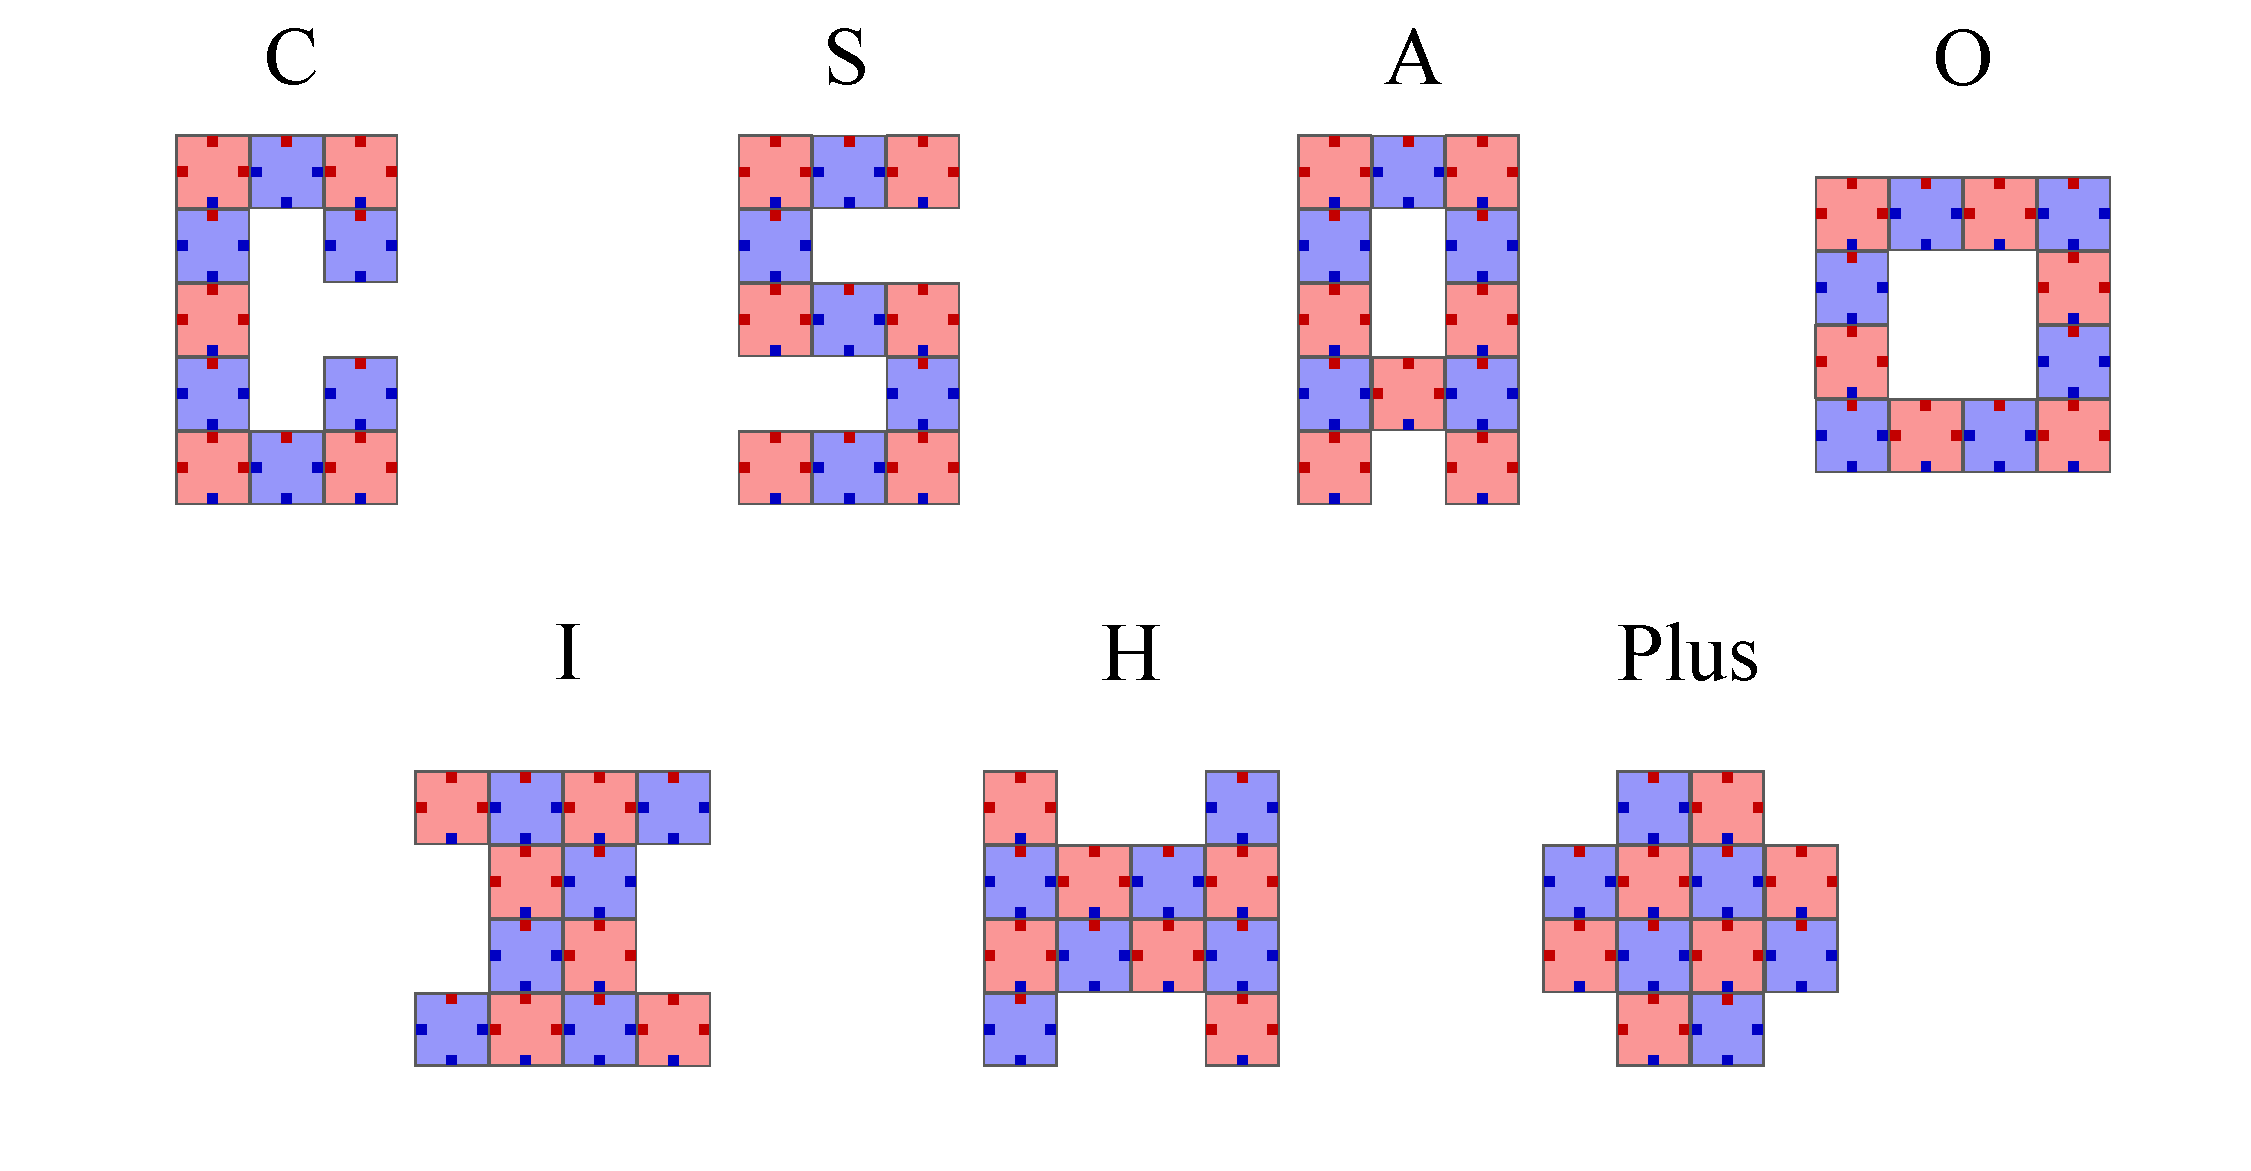
\includegraphics[width=0.8\textwidth]{figures/AFTS_sp_shapes.pdf}
		\caption{Special polyomino shapes evaluated in \autoref{sec:special_poly}.}
		\label{fig:AFTS_sp_shapes}
	\end{subfigure}
	\caption[List of manually designed polyominoes for experimenting]{List of manually designed polyominoes for experimenting.}
	\label{fig:AFTS_shapes}
\end{figure}

In this experiment manually designed polyominoes are assembled from multiple randomly generated initial configurations.
$100$ samples were taken for each custom polyomino with a workspace size of $50 r_C \times 50 r_C$.

In \autoref{sec:w/h_pattern} we focus on how rectangular polyominoes with varying width/height ratios influence planning time.
Furthermore we experiment with two patterns of red and blue for each rectangle.
The \textit{switching-column pattern} switches between red and blue cubes column vise and the \textit{checkerboard pattern} creates a checkerboard of single red and blue cubes.
A list of these polyominoes can be found in \autoref{fig:AFTS_cb_shapes}.

In \autoref{sec:special_poly} assembly of special polyomino shapes is examined. 
The polyominoes are listed in \autoref{fig:AFTS_sp_shapes}.
The polyominoes ``letter C'', ``letter S'' and ``letter A'' provide different caves.
``letter A'' additionally contains a hole. 

\subsection{Width/Height and Cube Pattern}
\label{sec:w/h_pattern}




\begin{figure}
	\centering
	\begin{subfigure}[b]{\textwidth}
		\centering
		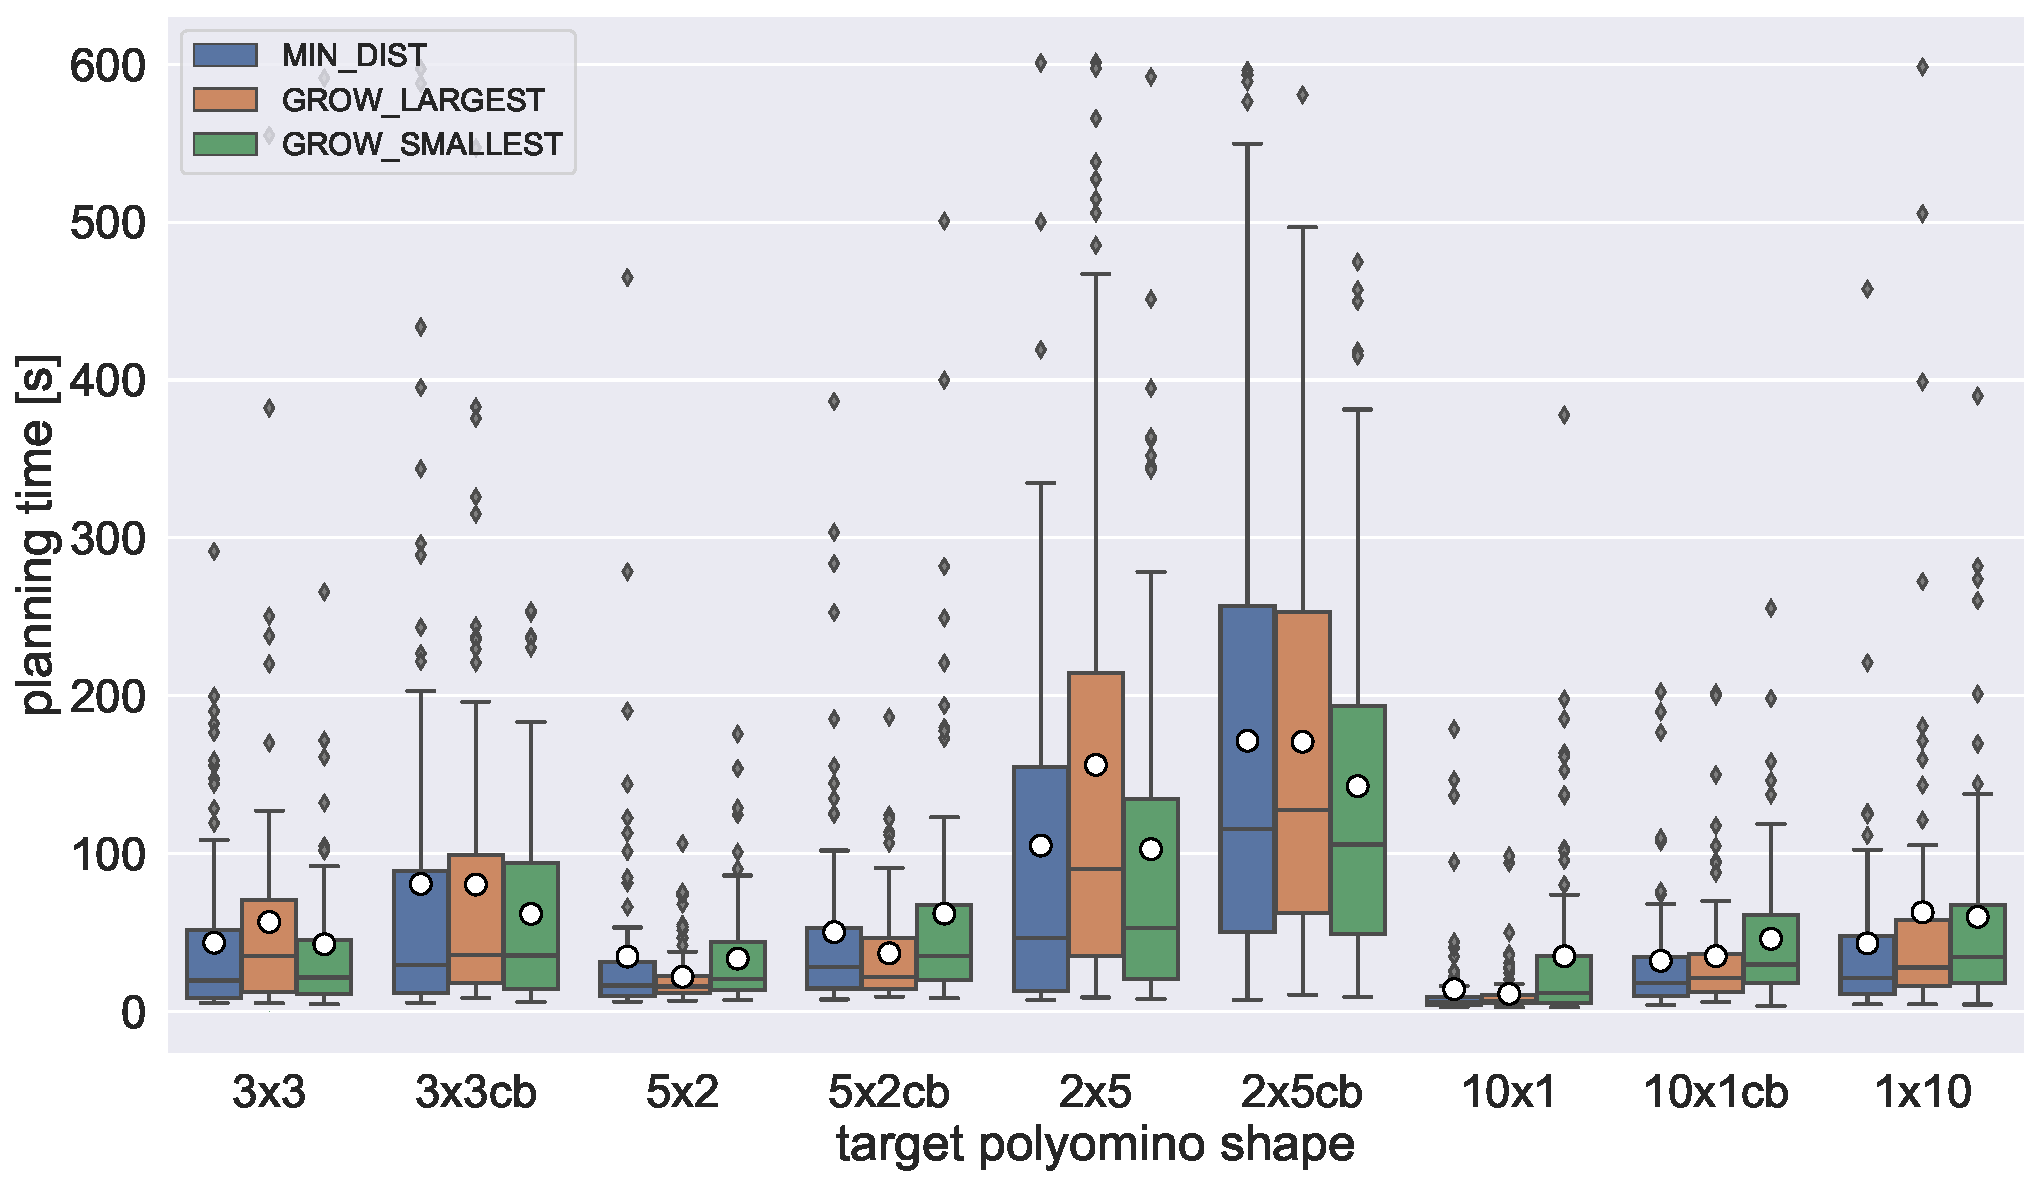
\includegraphics[width=0.9\textwidth]{figures/plots/AFTS_cb_time.pdf}
		\caption{}
		\label{fig:AFTS_cb_time}
	\end{subfigure}
	
	\begin{subfigure}[b]{\textwidth}
		\centering
		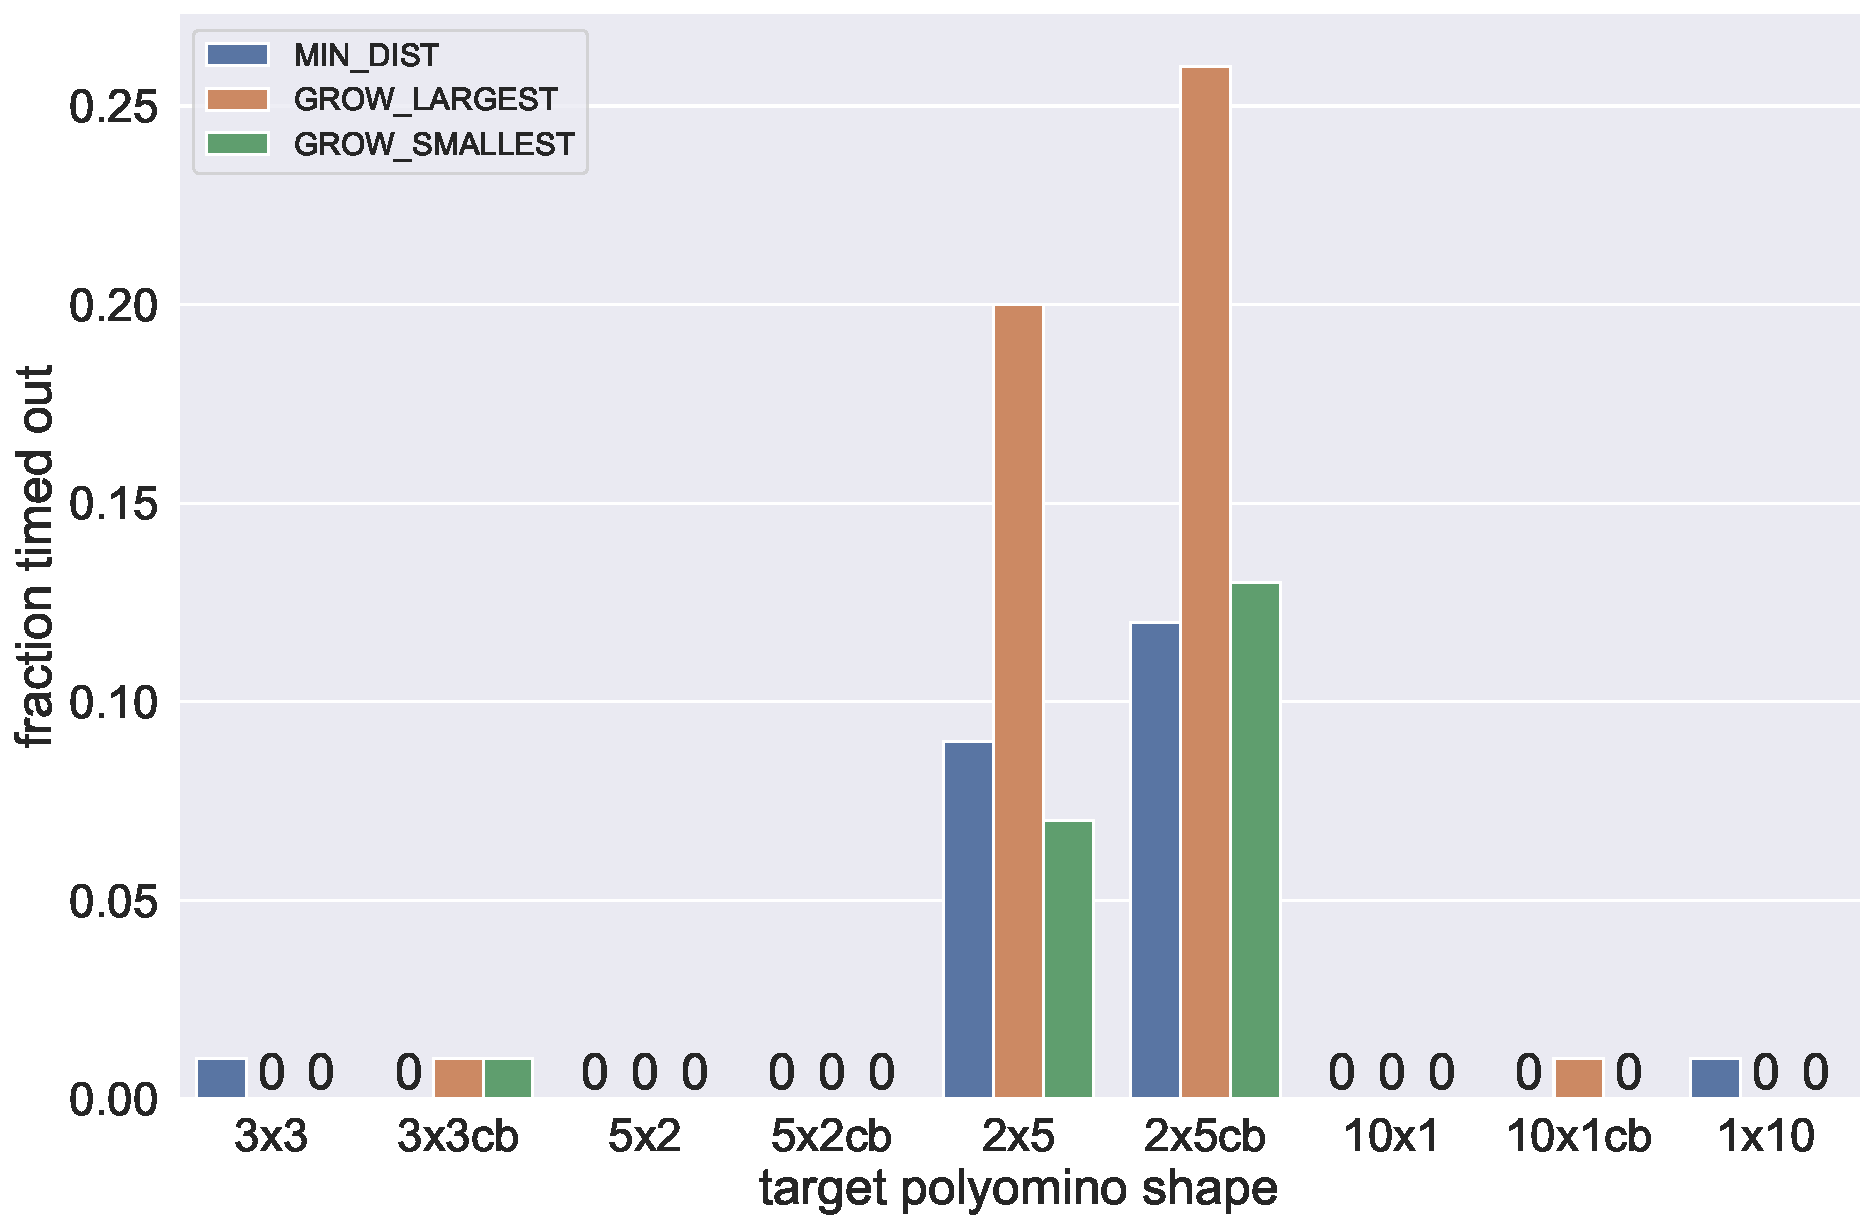
\includegraphics[width=0.9\textwidth]{figures/plots/AFTS_cb_timeout.pdf}
		\caption{}
		\label{fig:AFTS_cb_timeout}
	\end{subfigure}
	\caption[]{}
	\label{fig:AFTS_cb_timestats}
\end{figure}

Text


\subsection{Special Polyomino Shapes}
\label{sec:special_poly}


\begin{figure}
	\centering
	\begin{subfigure}[b]{\textwidth}
		\centering
		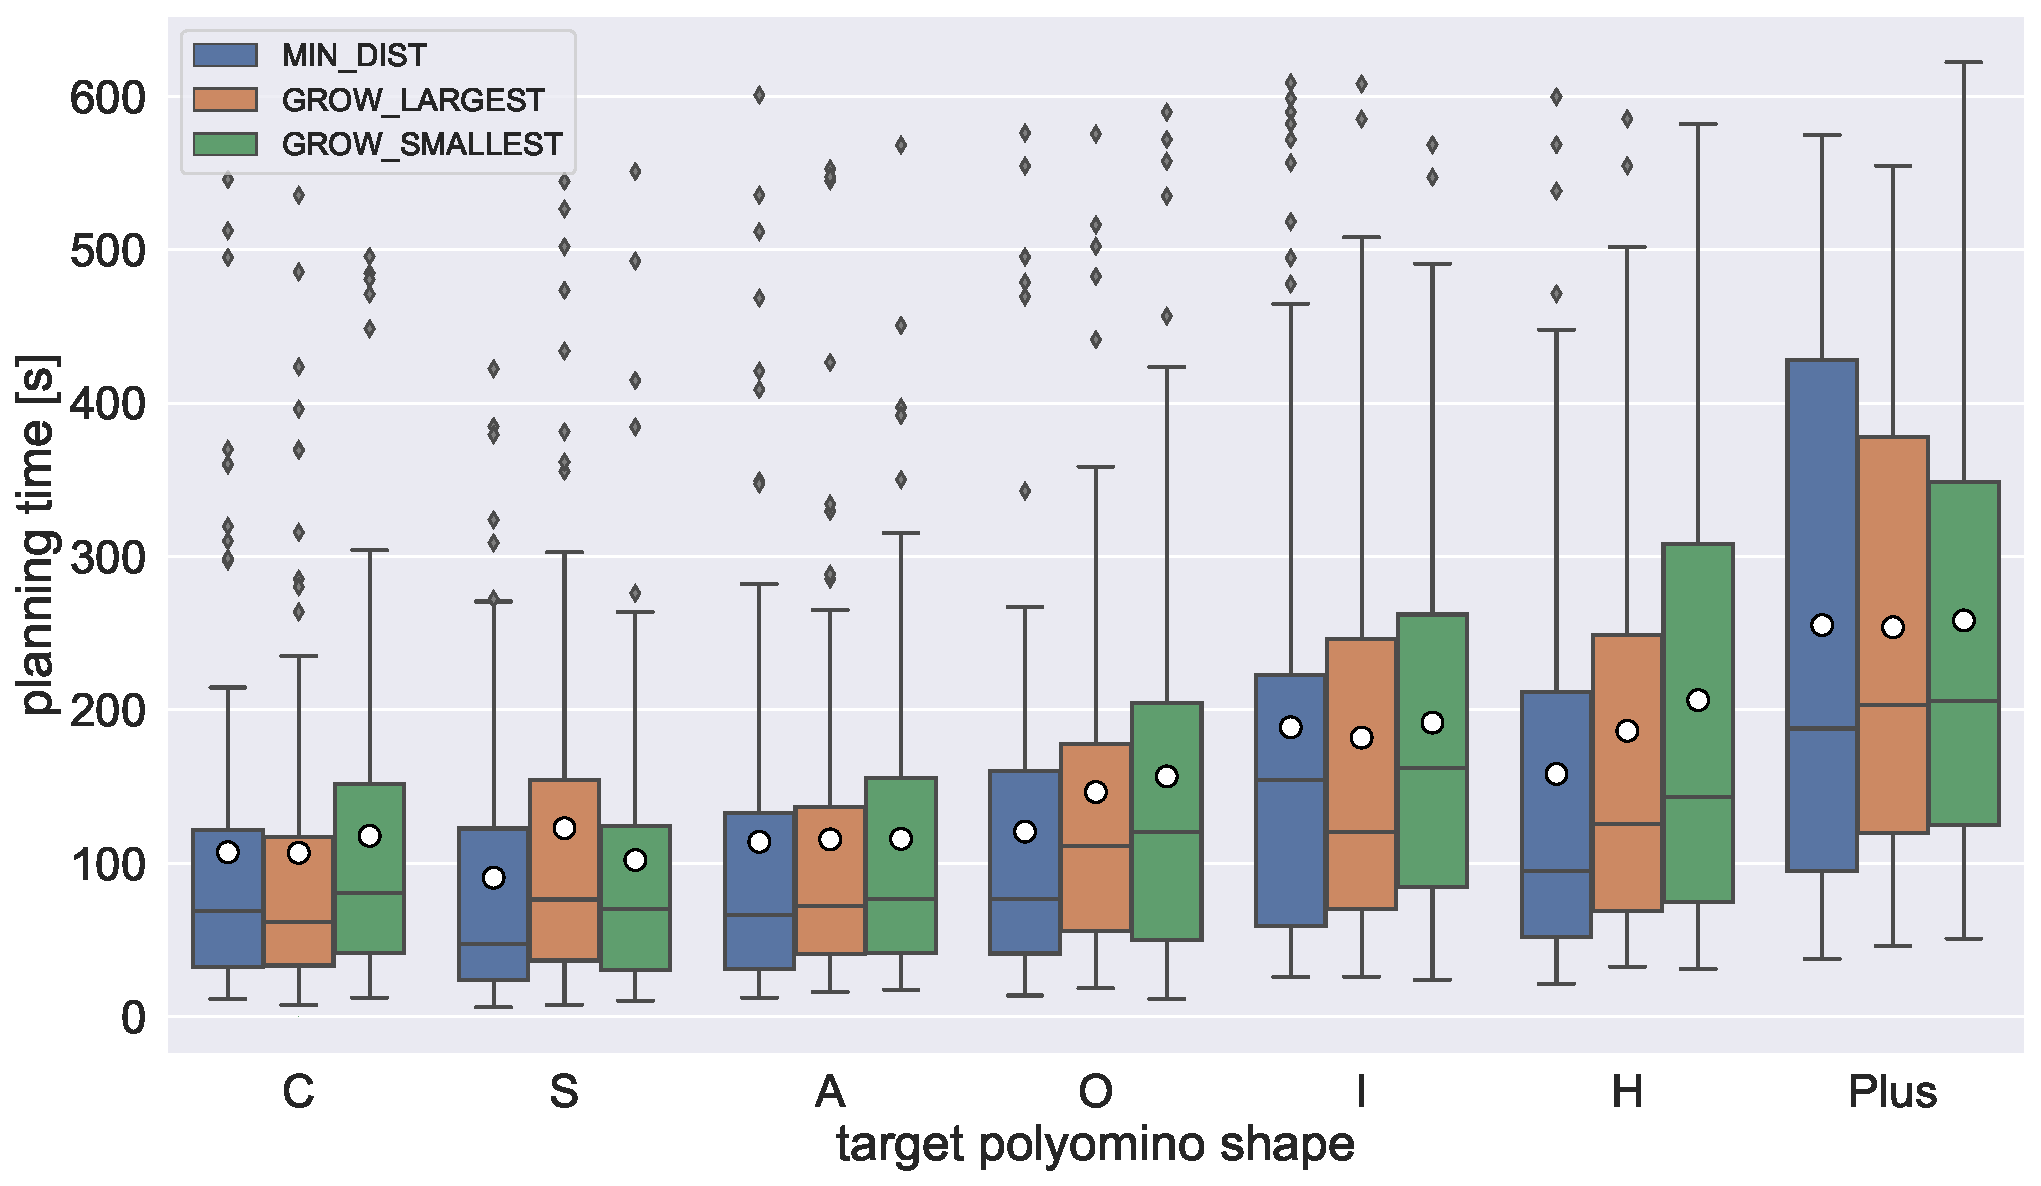
\includegraphics[width=0.9\textwidth]{figures/plots/AFTS_sp_time.pdf}
		\caption{}
		\label{fig:AFTS_sp_time}
	\end{subfigure}
	
	\begin{subfigure}[b]{\textwidth}
		\centering
		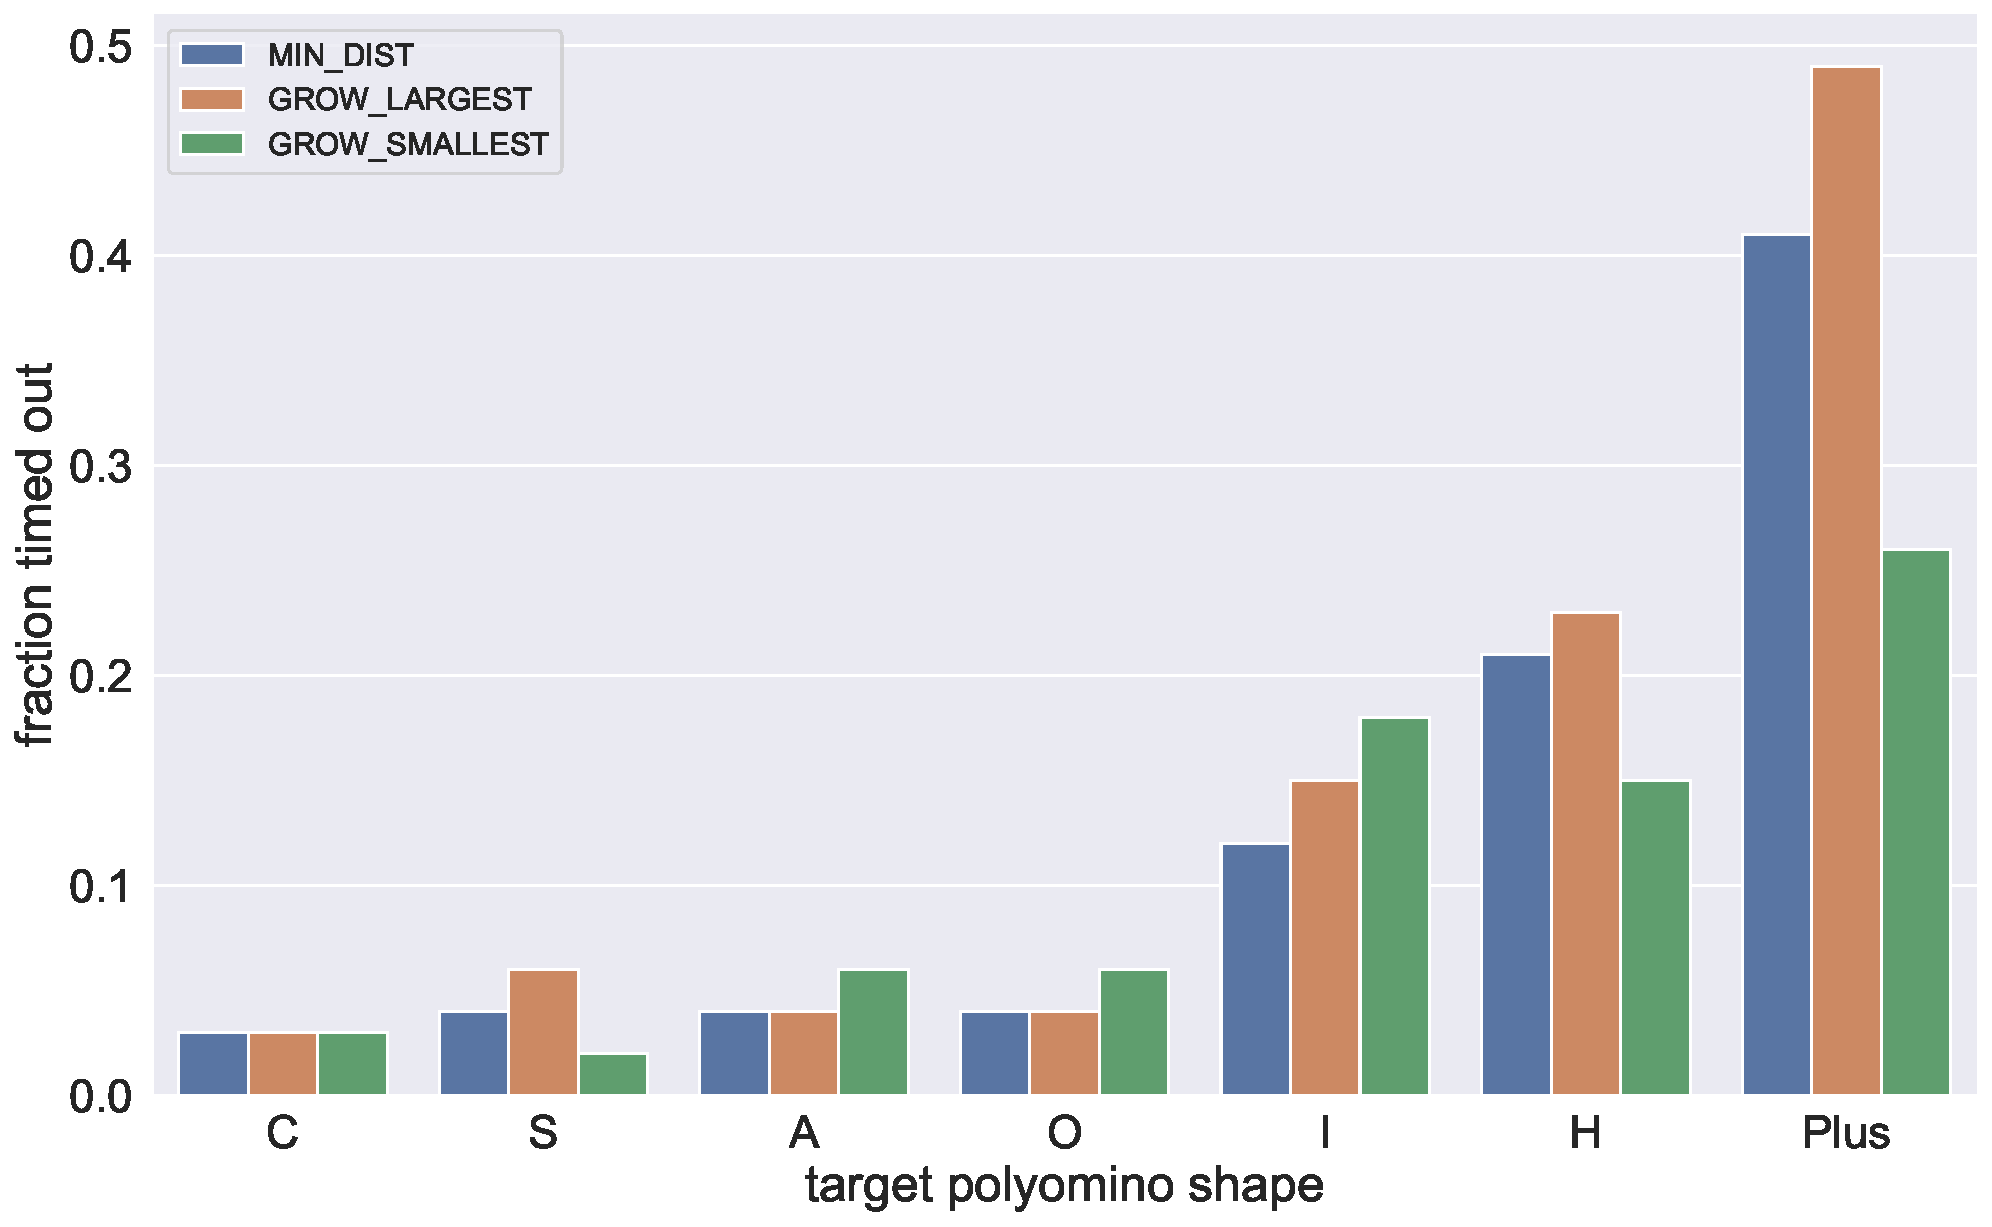
\includegraphics[width=0.9\textwidth]{figures/plots/AFTS_sp_timeout.pdf}
		\caption{}
		\label{fig:AFTS_sp_timeout}
	\end{subfigure}
	\caption[]{}
	\label{fig:AFTS_sp_timestats}
\end{figure}

Text




\section{Assembly for Workspace Size}
\label{sec:AFBS}

\begin{figure}
	\centering
	\begin{subfigure}[b]{\textwidth}
		\centering
		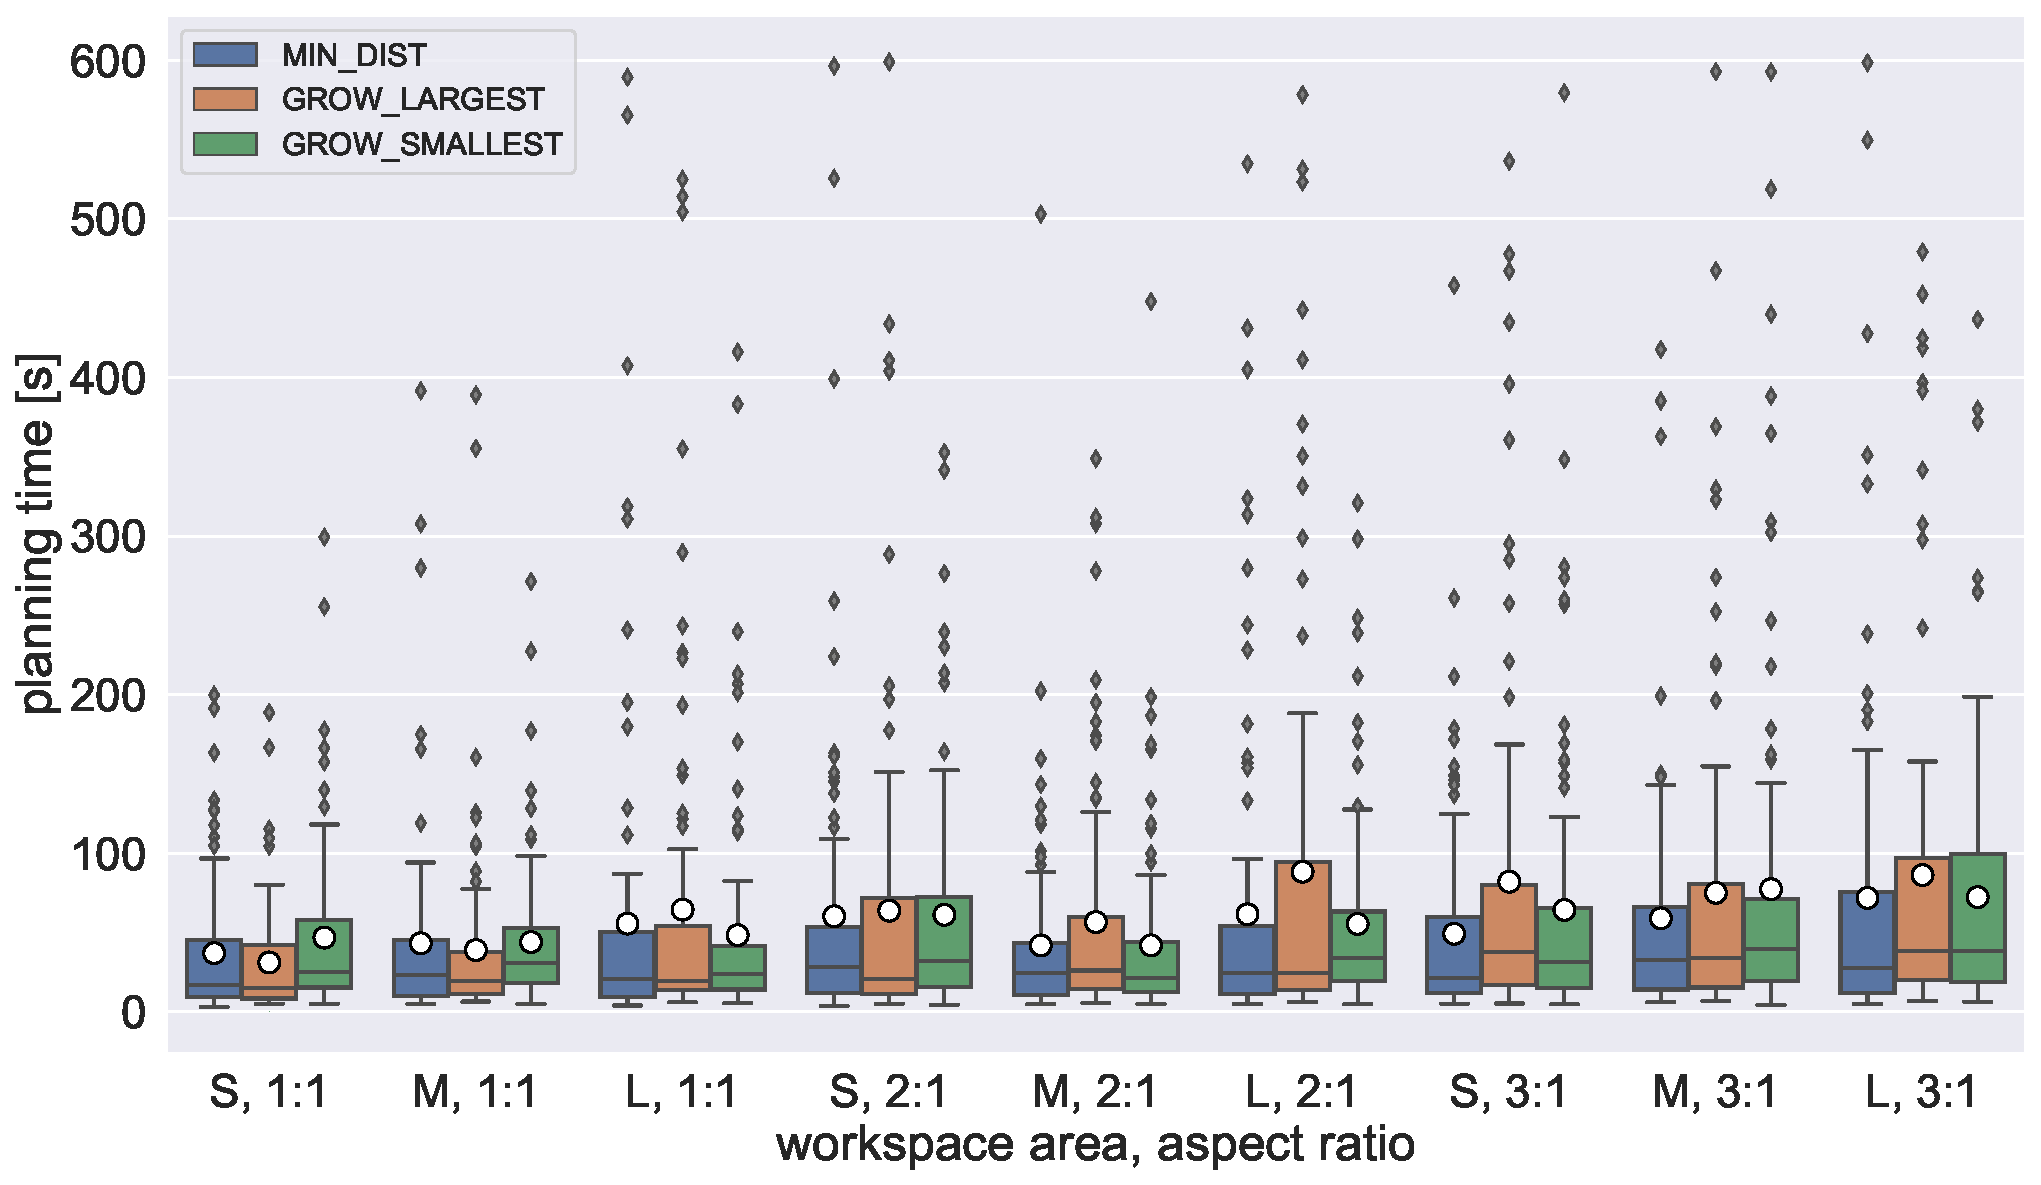
\includegraphics[width=0.9\textwidth]{figures/plots/AFBS_time.pdf}
		\caption{}
		\label{fig:AFBS_time}
	\end{subfigure}
	
	\begin{subfigure}[b]{\textwidth}
		\centering
		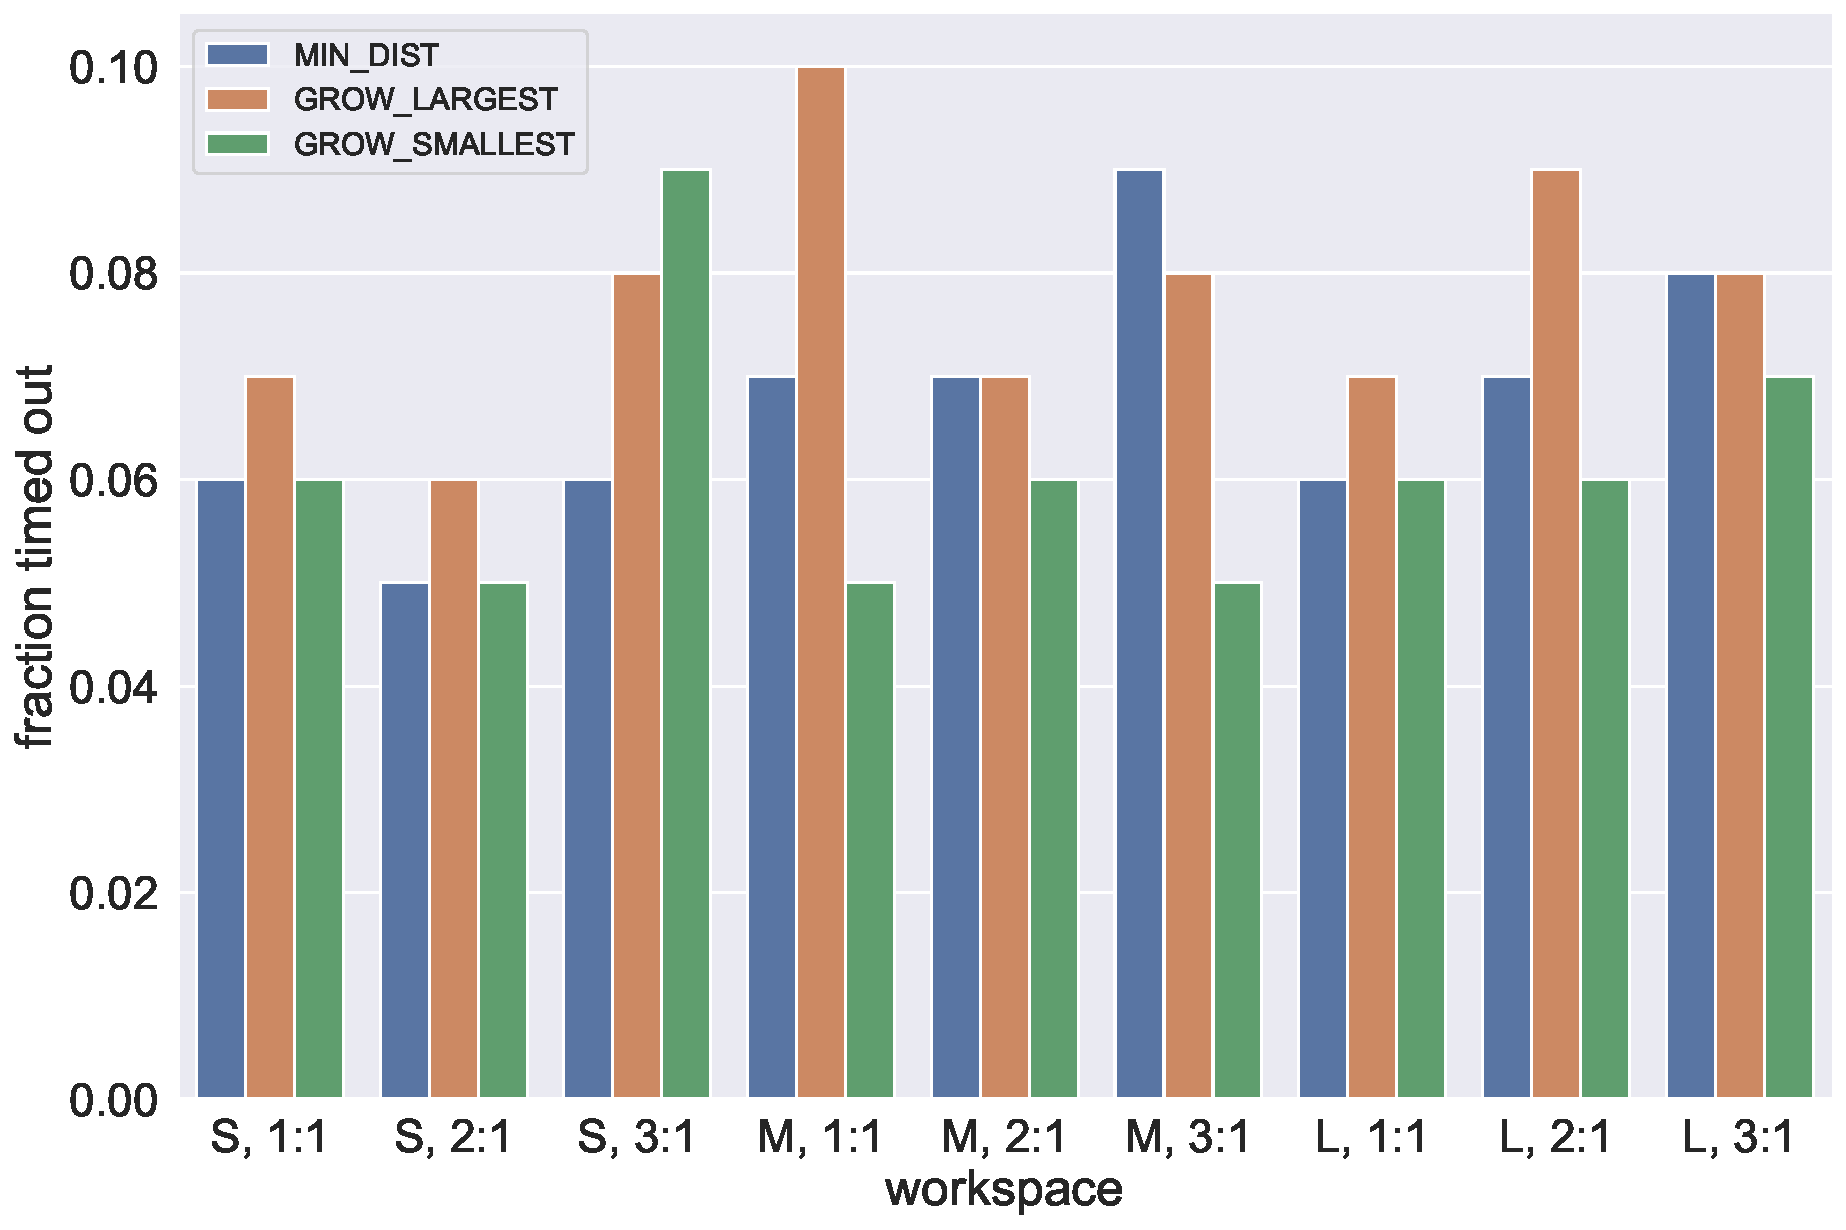
\includegraphics[width=0.9\textwidth]{figures/plots/AFBS_timeout.pdf}
		\caption{}
		\label{fig:AFBS_timeout}
	\end{subfigure}
	\caption[]{}
	\label{fig:AFBS_timestats}
\end{figure}

\begin{figure}
	\centering
	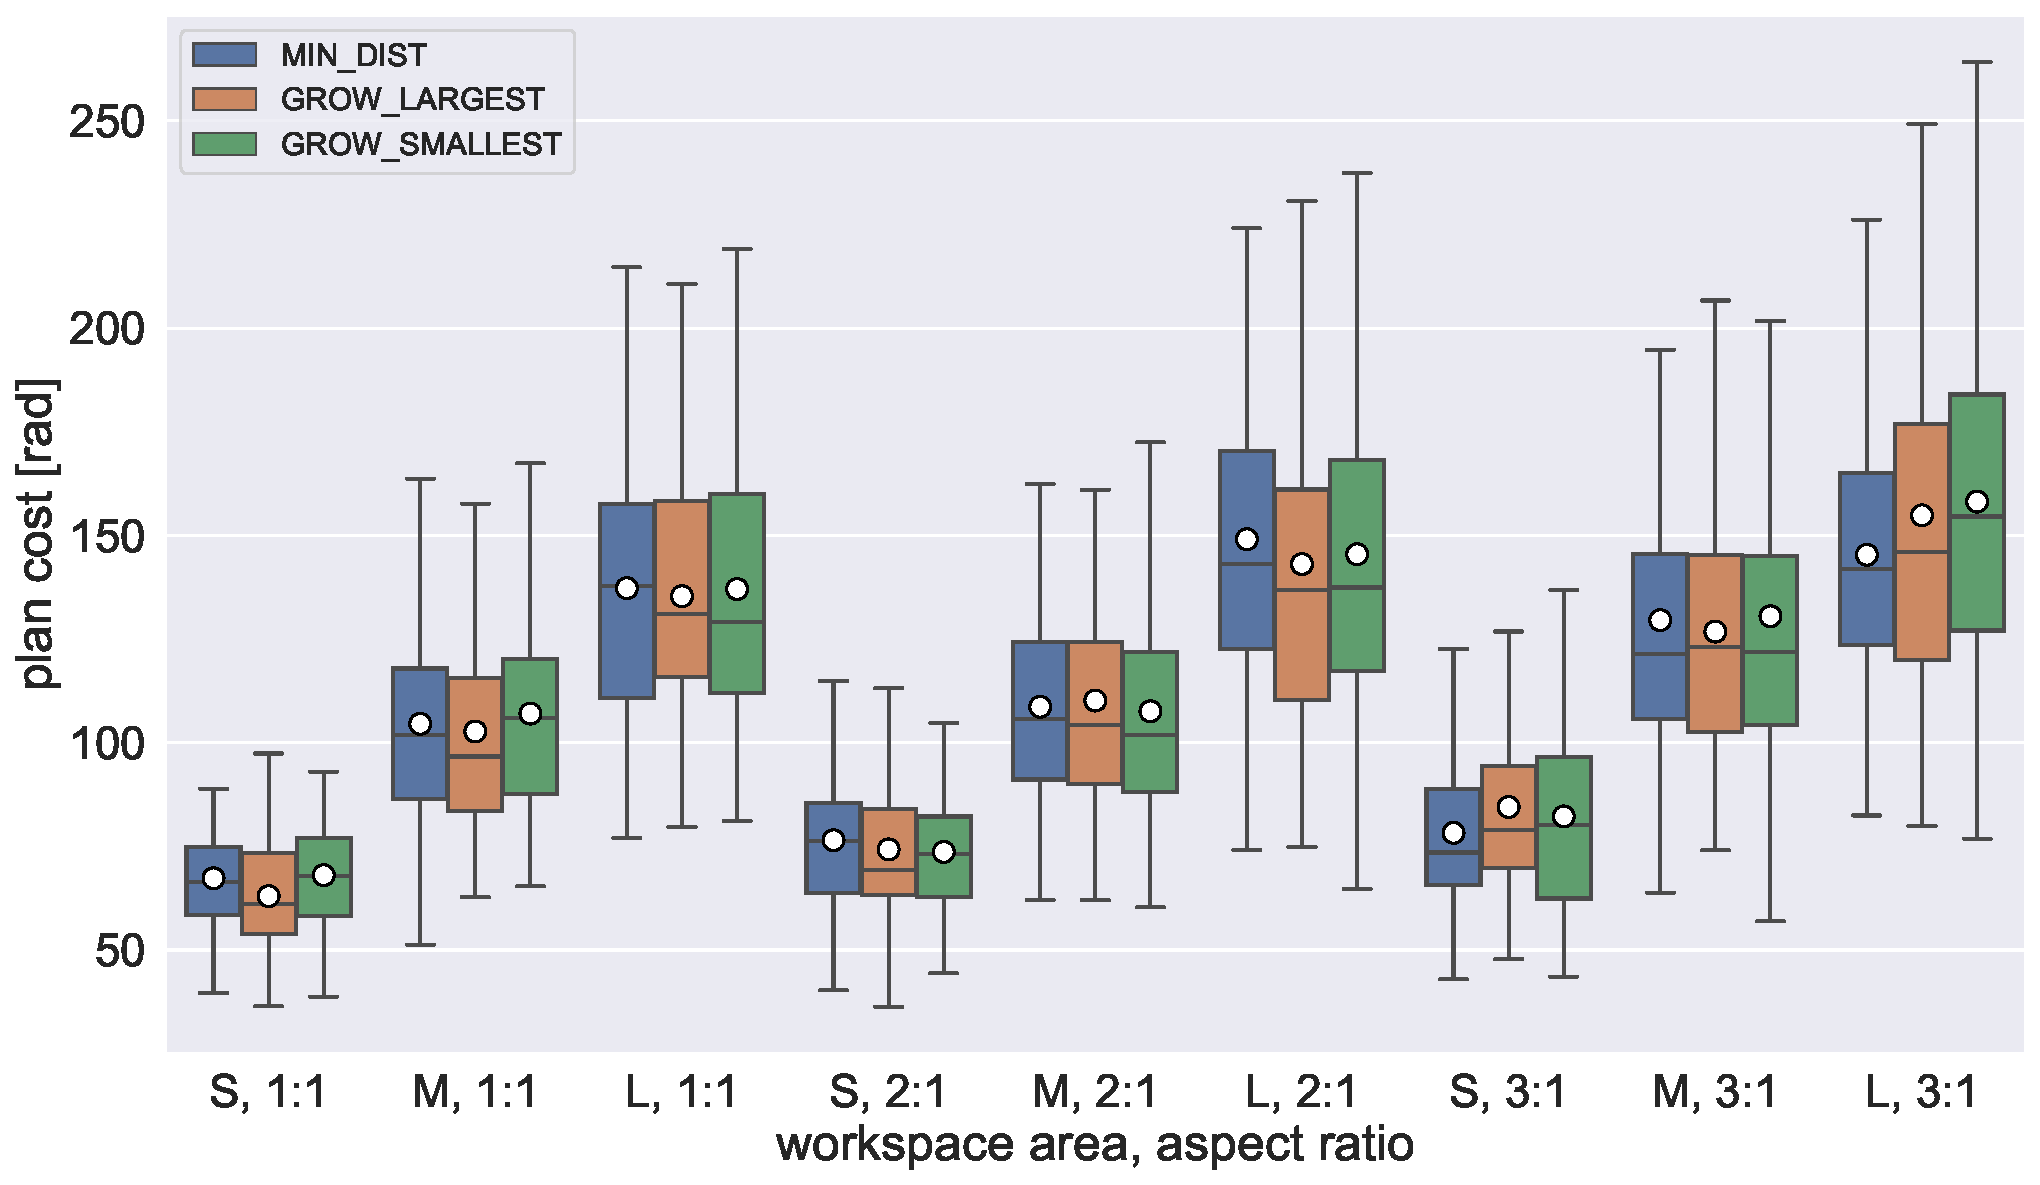
\includegraphics[width=0.9\textwidth]{figures/plots/AFBS_cost.pdf}
	\caption[]{}
	\label{fig:AFBS_cost}
\end{figure}

Text


\section{Assembly for Red to Blue Ration}
\label{sec:AFNR}



